\documentclass[12pt]{article}
\usepackage{amsmath}
\usepackage{graphicx}
\usepackage{caption}
\usepackage{subcaption}
\usepackage{booktabs}
\usepackage{float}
\usepackage[utf8]{inputenc}
\usepackage{geometry}
\usepackage{multirow}
\usepackage{setspace}
\usepackage{parskip}
\usepackage{svg}
\usepackage[bottom]{footmisc}
\usepackage{tikz}
\usepackage[section]{placeins}
\usepackage{enumitem}
\usepackage{listings}
\usepackage{tikz}
\usepackage{enumitem}
% \usepackage{url}
\usepackage{xurl}

% Specify the serif font
% \setmainfont{Times New Roman}

% Define custom colors
\definecolor{codebackground}{rgb}{0.95,0.95,0.95}
\definecolor{codecomment}{rgb}{0,0.5,0}
\definecolor{codekeyword}{rgb}{0,0,1}
\definecolor{codestring}{rgb}{0.5,0,0.5}


% Define custom style for code listings
\lstdefinestyle{mystyle}{
    backgroundcolor=\color{codebackground},
    basicstyle=\ttfamily\small, % Choose your custom font and size
    commentstyle=\color{codecomment},
    keywordstyle=\color{codekeyword},
    stringstyle=\color{codestring},
    % numbers=left,
    numberstyle=\tiny,
    numbersep=5pt,
    breaklines=true,
    breakatwhitespace=true,
    captionpos=b,
    frame=single,
    framesep=5pt,
    rulecolor=\color{black},
    showspaces=false,
    showstringspaces=false,
    showtabs=false,
}

\lstset{style=mystyle}


% \lstset{%
%    frame=single,
%    framerule=1pt,
%    breaklines=true,
%    postbreak=\mbox{\textcolor{red}{$\hookrightarrow$}\space},
%    aboveskip=6pt, % Adjust the spacing above the code listing
%    belowskip=6pt  % Adjust the spacing below the code listing
% }
\setlength{\textfloatsep}{5pt}

% This style is used to create block diagrams, you'll find it useful since many of your figures would be of that form, I'll try add more styles in the future :)
\usetikzlibrary{trees,positioning,fit,calc}
\tikzset{block/.style = {draw, fill=blue!20, rectangle,
                         minimum height=3em, minimum width=4em},
        input/.style = {coordinate},
        output/.style = {coordinate}
}

\usepackage[section]{minted}
\usepackage{xcolor}
\usemintedstyle{porland}

\usepackage{chngcntr}
\counterwithin{figure}{section}

\renewcommand{\arraystretch}{1.5}

\usepackage[hidelinks]{hyperref}
\hypersetup{
    linktoc=all
}

\renewcommand\listingscaption{Listing}
\renewcommand\listoflistingscaption{List of Listings}

\usepackage{scrhack}
\usepackage{tocbasic}
\setuptoc{lol}{levelup}

\usepackage{indentfirst}
\geometry{a4paper, margin=1in}

%----------EDIT COVER INFO HERE -----------------%

\def \LOGOPATH {lnxiorem4uqo18zw8-General_ECOSYSTEMS_SpaceOrbit_Spot.svg}
\def \DEPARTEMENT {Department of Computer Science \& Engineering}
\def \COURSENUM {CSL7090}
\def \COURSENAME {Software \& Data Engineering (SDE)}
\def \REPORTTITLE {Course Project}
\def \STUDENTNAME {Aviral Tripathi \& Ritik Kumar}
\def \STUDENTID {STUDNUM}
\def \INSTRUCTOR {Dr. Sumit Kalra}

%------------------------------------------------%

\setlength{\parindent}{0em}
\setlength{\parskip}{0em}

\begin{document}

\pagenumbering{Roman}

\begin{titlepage}
    \vfill
    \begin{center}
        \includesvg[width=1\textwidth]{\LOGOPATH} \\
        \hfill \\
        \Large{\DEPARTEMENT} \\
        \Large{\COURSENUM\;-\;\COURSENAME} \\
        \vfill
        % {\fontfamily{ptm}\selectfont\textsc{\textbf{\LARGE{\REPORTTITLE}}}}

        % \usepackage{graphicx}

% ...

        \resizebox{1\textwidth}{!}{%
          {\fontfamily{ptm}\selectfont\textsc{{\small{\REPORTTITLE}}}}%
        }
    \end{center}
    \vfill
    \begin{flushleft}
        \Large{\textbf{Prepared by:} \STUDENTNAME} \\
        \Large{\textbf{Roll no:} m22ma012 \& m22ma009} \\
        \Large{\textbf{Instructor:} \INSTRUCTOR}
    \end{flushleft}
    \vfill
\end{titlepage}

%--------------ABSTRACT ------------------------%
{
%\centering
%\section*{Abstract}
%You can check the \mintinline{text}{cites.bib} in order to add references (it would be automatically added to the report once you cite it\cite{rfc3447} with \mintinline{latex}{\cite{tag}}). For the figures I do not prefer static figures, I like to generate them with TikZ, but in case you've needed some static figures you can add them to the \mintinline{text}{assets} directory to keep your files organized.
%\clearpage
}

%-----------------------------------------------%

\tableofcontents
\clearpage

\setlength{\parskip}{\baselineskip}%

\pagenumbering{arabic}

%--------------INTRODUCTION ---------------------%

\section{Research Paper}
\subsection{Node.js: Using JavaScript 
to Build High-Performance 
Network Programs (IEEE)}


\begin{figure}[H]
    \centering
    \includegraphics[width=0.1\textwidth]{assets/nodejs-logo-FBE122E377-seeklogo.com.png}
    \caption{Node JS}
    \label{fig:logo}
\end{figure}


The paper explains about the working of Node JS along with its various advantages and how it compares with the 'Multi-threaded Environments', here are some key points from the paper:

\begin{itemize}[noitemsep]
  \itemsep0.5em
  
  \item Node JS is a server-side JavaScript environment, for long running server processes.
  \item It uses the asynchronous event model i.e there is only one thread that is processed at one time (unlike multi-threaded environments where multiple threads can be processed at one time), by switching between different threads for code execution.
  \item When one thread is busy the processor jumps to another thread
  % \item Operating System: Ubuntu: chosen because of familiarity with CLI commands
  % \item Storage: 50GB
  
\end{itemize}

The need for an Asynchronous Event based environment arised because of the disadvantages of multi-threaded environments: 

\begin{itemize}[noitemsep]
  \itemsep0.5em
  
  \item Deadlock between threads on shared resources
  \item Less control to developer, as OS itself decides which thread to exec and for how long
  % \item 
  
\end{itemize}

\textbf{Example for the working of Node JS}

\hspace{1cm} If the application writes to a socket and fills the socket’s underlying buffer, ordinarily, the socket blocks the application’s writes until buffer space becomes available, thus preventing the application from doing any other useful work. 

\hspace{1cm} But, if the socket is non-blocking, it instead returns an indication to the application that further writing isn’t currently possible, thereby informing the application that it should try again later. Assuming the application has registered interest with the event notification system in that socket, it can go do something else, knowing that it will receive an event when the socket’s write buffer 
has available space.

% why JavaScript is popular: “HTML 5” reduces 
% the appeal of alternative client-side 
% platforms, NoSQLtype databases such as CouchDB 
% and Riak use JavaScript, high-performance 
% JavaScript runtime implementations 
% that are extremely fast and scalable.

\begin{itemize}[noitemsep]
  \itemsep0.5em
  
  \item JavaScript is a functional language and, as such, supports higher-order functions.

  \item Every I/O operation is handled by means of higher-order functions — i.e, functions taking functions as a parameter — that specify what to do when there’s something to do. 

  % \item 
  
\end{itemize}

\clearpage

\begin{listing}[h]
\begin{minted}[frame=single,framesep=10pt,breaklines,breakanywhere]{shell}
var sys = require(“sys”),
	http = require(“http”),
	url = require(“url”),
 	path = require(“path”),
 	fs = require(“fs”);
http.createServer(function(request, response) {
	var uri = url.parse(request.url).pathname;
 	var filename = path.join(process.cwd(), uri);
 	path.exists(filename, function(exists) {
 		if(exists) {
 			fs.readFile(filename, function(err, data) {
 				response.writeHead(200);
 				response.end(data);
 			});
		} else {
 			response.writeHead(404);
 			response.end();
 	   }
 	});
}).listen(8080);
sys.log(“Server running at http://localhost:8080/”);


\end{minted}
\end{listing}

\begin{center}
\textbf{A simple HTTP file server.}
\end{center}

% \clearpage

\begin{itemize}[noitemsep]
  \itemsep0.5em
  
  \item The http \textbf{createServer()} function, which is a wrapper around a low-level efficient HTTP protocol implementation, is passed a function as the only argument. 

  \item This function is invoked whenever data for a new request is ready to be read. Node offers no opportunity to read a file synchronously — the only option is to register another function via \textbf{readFile()} that gets invoked whenever data can be read.


  % \item 
  
\end{itemize}



\begin{figure}[H]
    \centering
    \includegraphics[width=0.7\textwidth]{assets/nodejs2.png}
    \caption{Node JS Event Loop}
    \label{fig:logo}
\end{figure}









\section{Introduction}
\subsection{MERN Stack}
\vspace{1cm}
\begin{figure}[H]
    \centering
    \includegraphics[width=0.7\textwidth]{assets/MERN-logo.png}
    \caption{MERN Stack}
    \label{fig:logo}
\end{figure}


MERN stack is a technology stack comprising of:
\begin{itemize}[noitemsep]
  \itemsep0.5em
  
  \item MongoDB Database: for storing data
  \item Express JS: for backend and Routes
  \item React: for frontend
  \item Node JS: JavaScript execution environment (backend)
  
\end{itemize}

\subsubsection{\textbf{Mongo DB}}
It is a cloud based database service that can be used to store the data such as text, username, passwords, and files, we will be using this database to store the Post contents and user data such as username and passwords.

\subsubsection{Express JS:}
It helps in creating routes (URLs) and handle requests and responses. It makes it easier to manage the server-side logic of your application.

\subsubsection{React:}
It is used to build the frontend or the user interface of a website

\subsubsection{Node JS:}
It enables you to use JavaScript not only for frontend development but also for server-side development, in an asynchronous manner.



\section{Installations}

\subsection{Installing Node.JS}
To install node.js, got to the official website of Node, and install the .msi installation file for windows installation. After the download follow the steps of installation wizard to install node.

\begin{figure}[H]
    \centering
    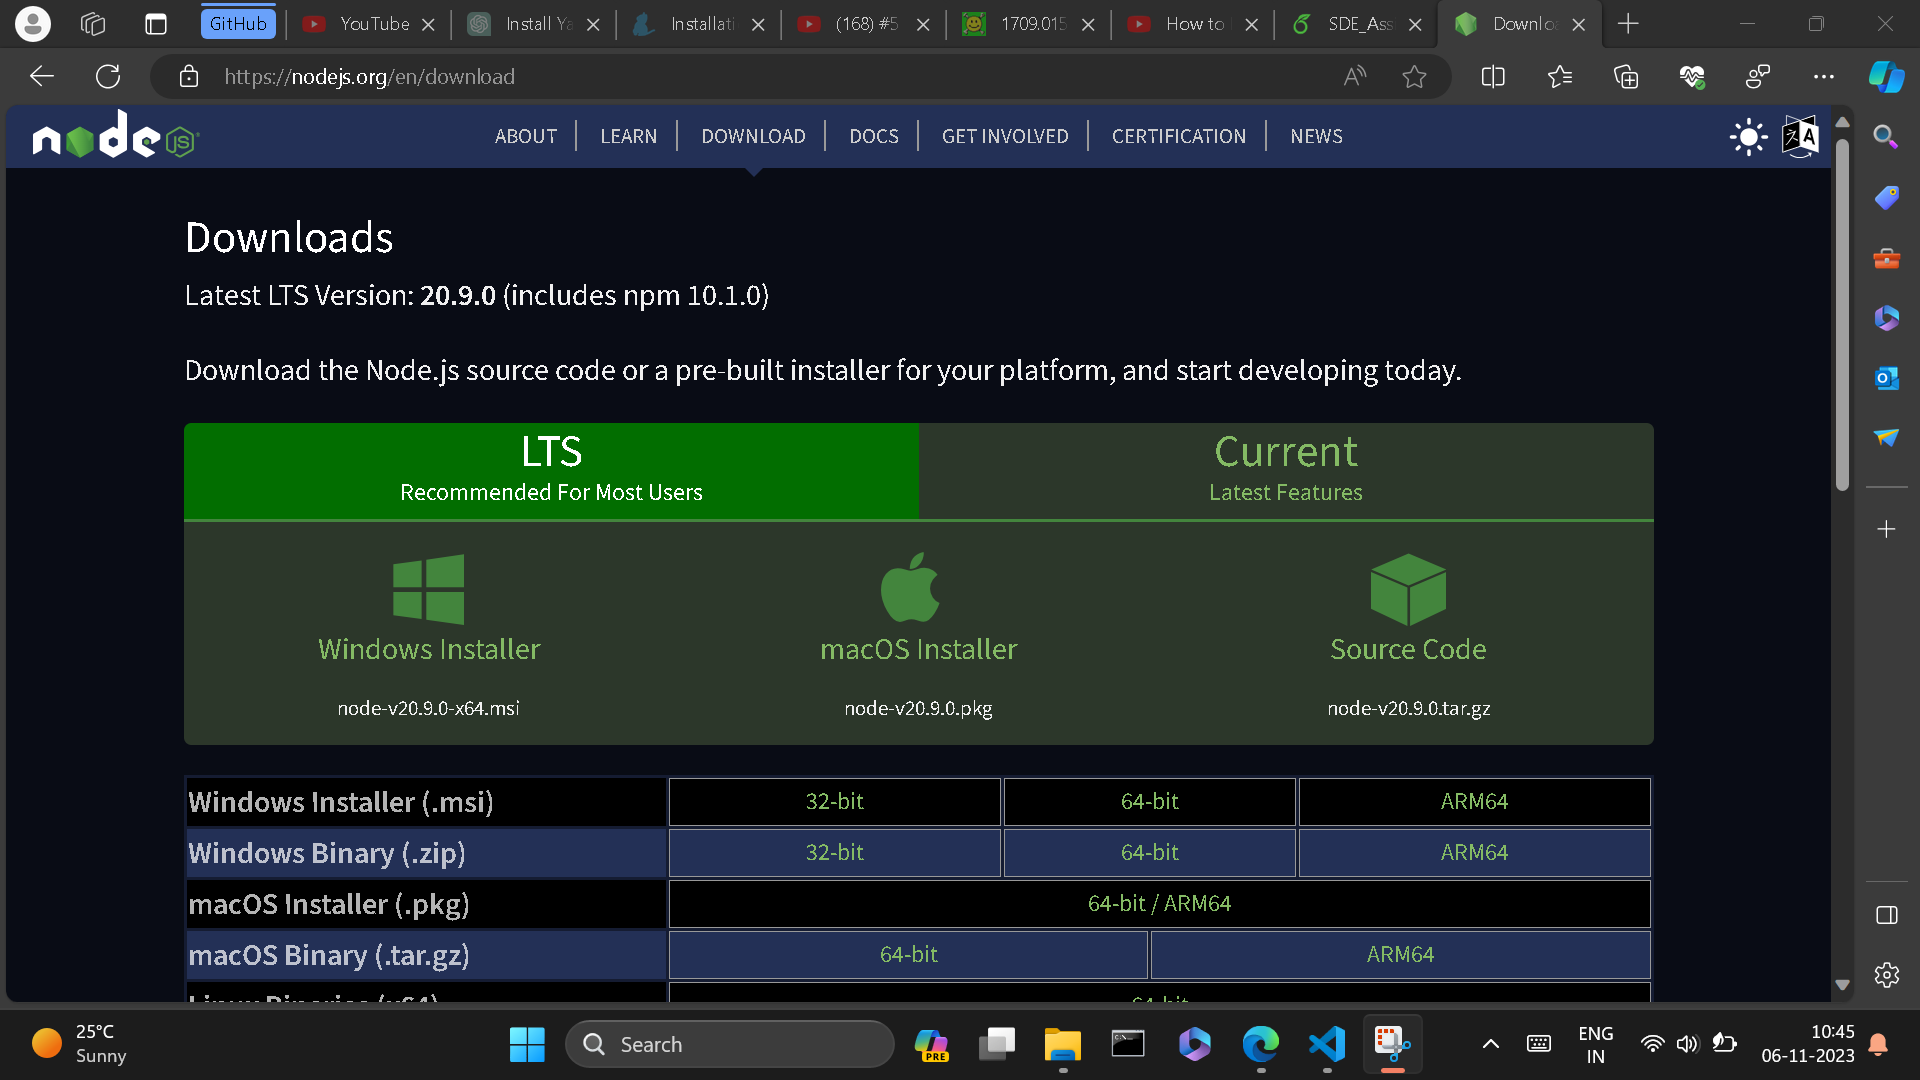
\includegraphics[width=1.0\textwidth]{assets/Node-officialWebsite.png}
    \caption{Node JS download}
    \label{fig:logo}
\end{figure}

\begin{figure}[H]
    \centering
    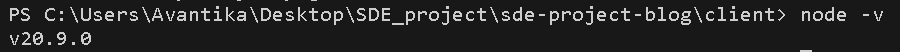
\includegraphics[width=1.0\textwidth]{assets/node-version.png}
    \caption{Verifying Node JS installation}
    \label{fig:logo}
\end{figure}

\subsection{Initialising a new React project.}
To initialise a new react project (web-app) we need to run the following commands

\begin{listing}[htbp]
\begin{minted}[frame=single,framesep=10pt,breaklines,breakanywhere]{shell}
Set-ExecutionPolicy -Scope CurrentUser RemoteSigned
yarn create react-app .
\end{minted}
\end{listing}

The first command is used to change the execution policy for the current user (scripts and configuration files that can be run for current user), the RemoteSigned keyword allows to download the scripts without requiring a digital signature

The second command is to define the predefined structure and configuration of a react app (the dot in the end signifies the current directory) and also install the required dependencies, and provides a basic app template overall.

% \begin{itemize}[noitemsep]
%   \itemsep0.5em
%   \item Location: Default
%   \item Type: E2-micro (0.25-2 vCPU, 1 shared core): chosen to reduce cost
%   \item RAM: 1GB
%   \item Operating System: Ubuntu: chosen because of familiarity with CLI commands
%   \item Storage: 50GB
% \end{itemize}

\begin{figure}[H]
    \centering
    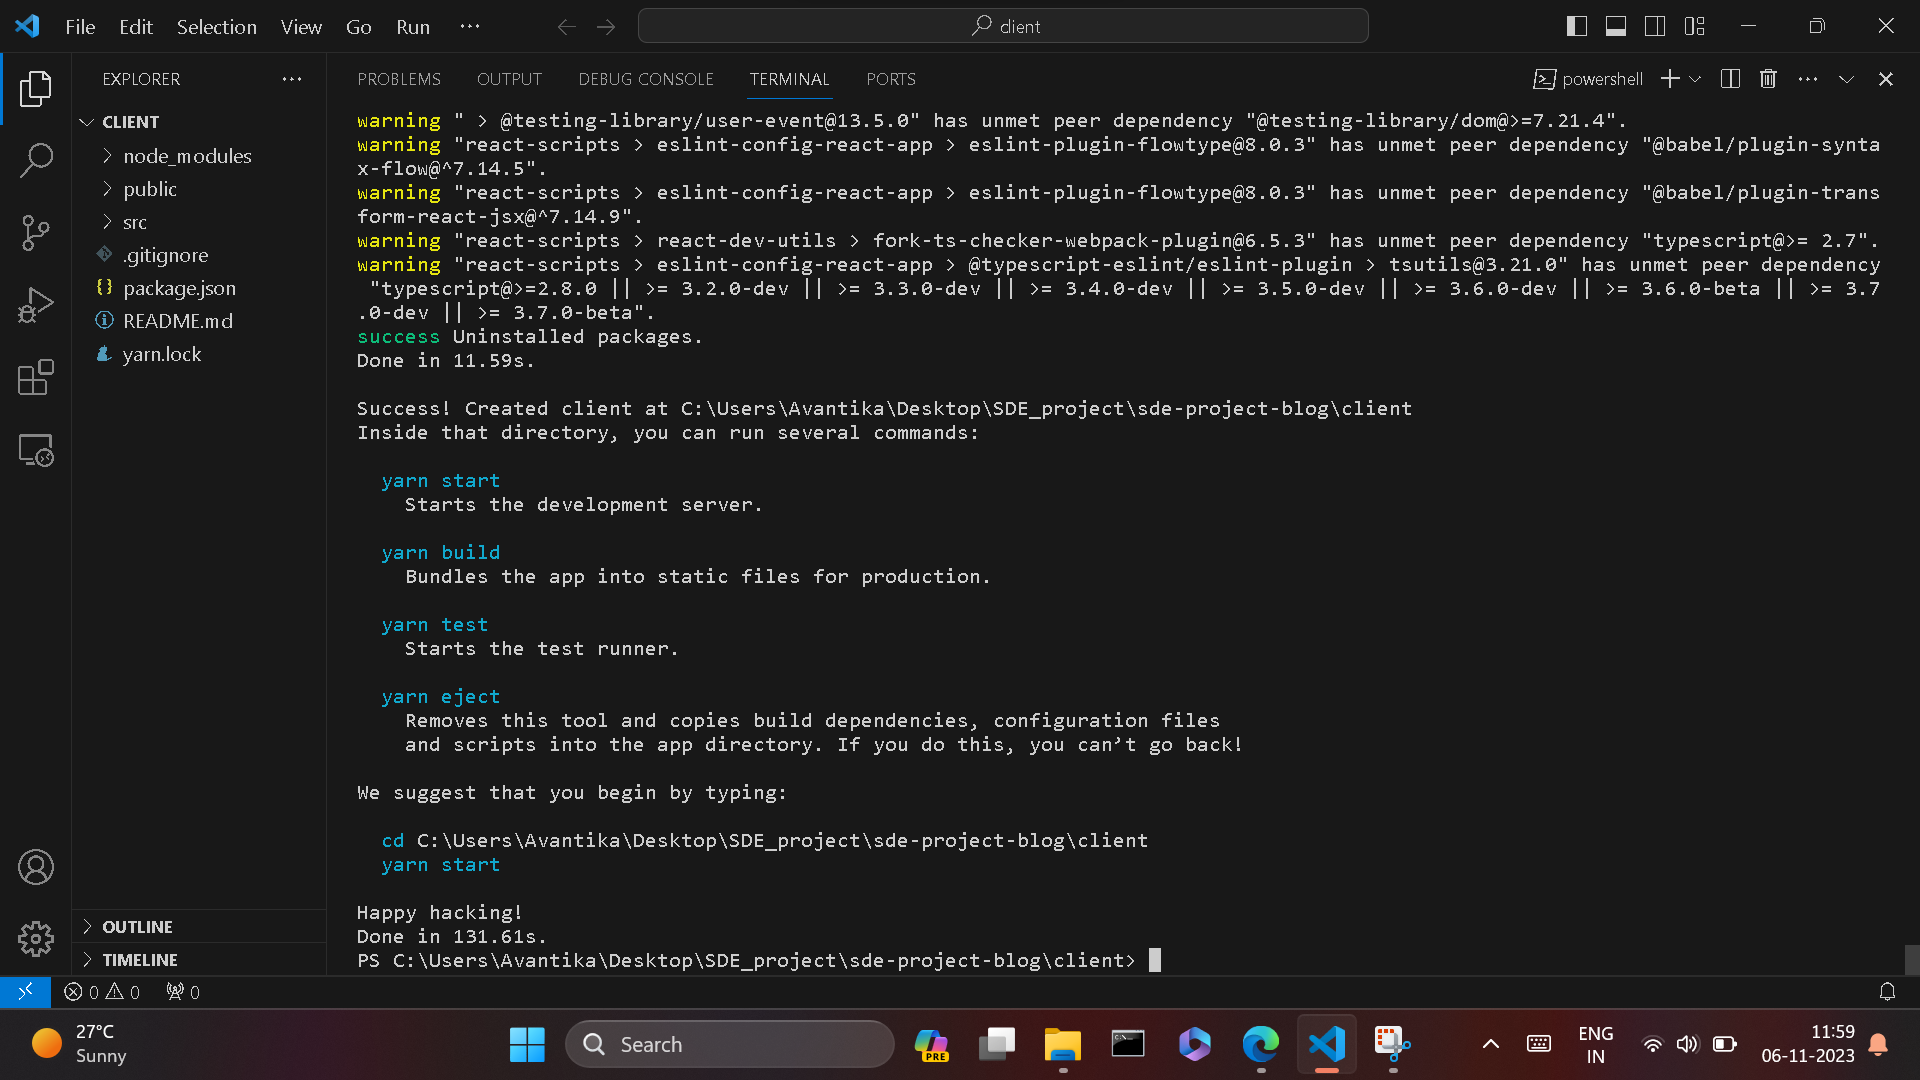
\includegraphics[width=1\textwidth]{assets/React-app-yarn-insatll.png}
    \caption{Create React App (CRA)}
    \label{fig:logo}
\end{figure}

To start the react app run the command:

\begin{listing}[htbp]
\begin{minted}[frame=single,framesep=10pt,breaklines,breakanywhere]{shell}
yarn start
\end{minted}
\end{listing}


\begin{figure}[H]
    \centering
    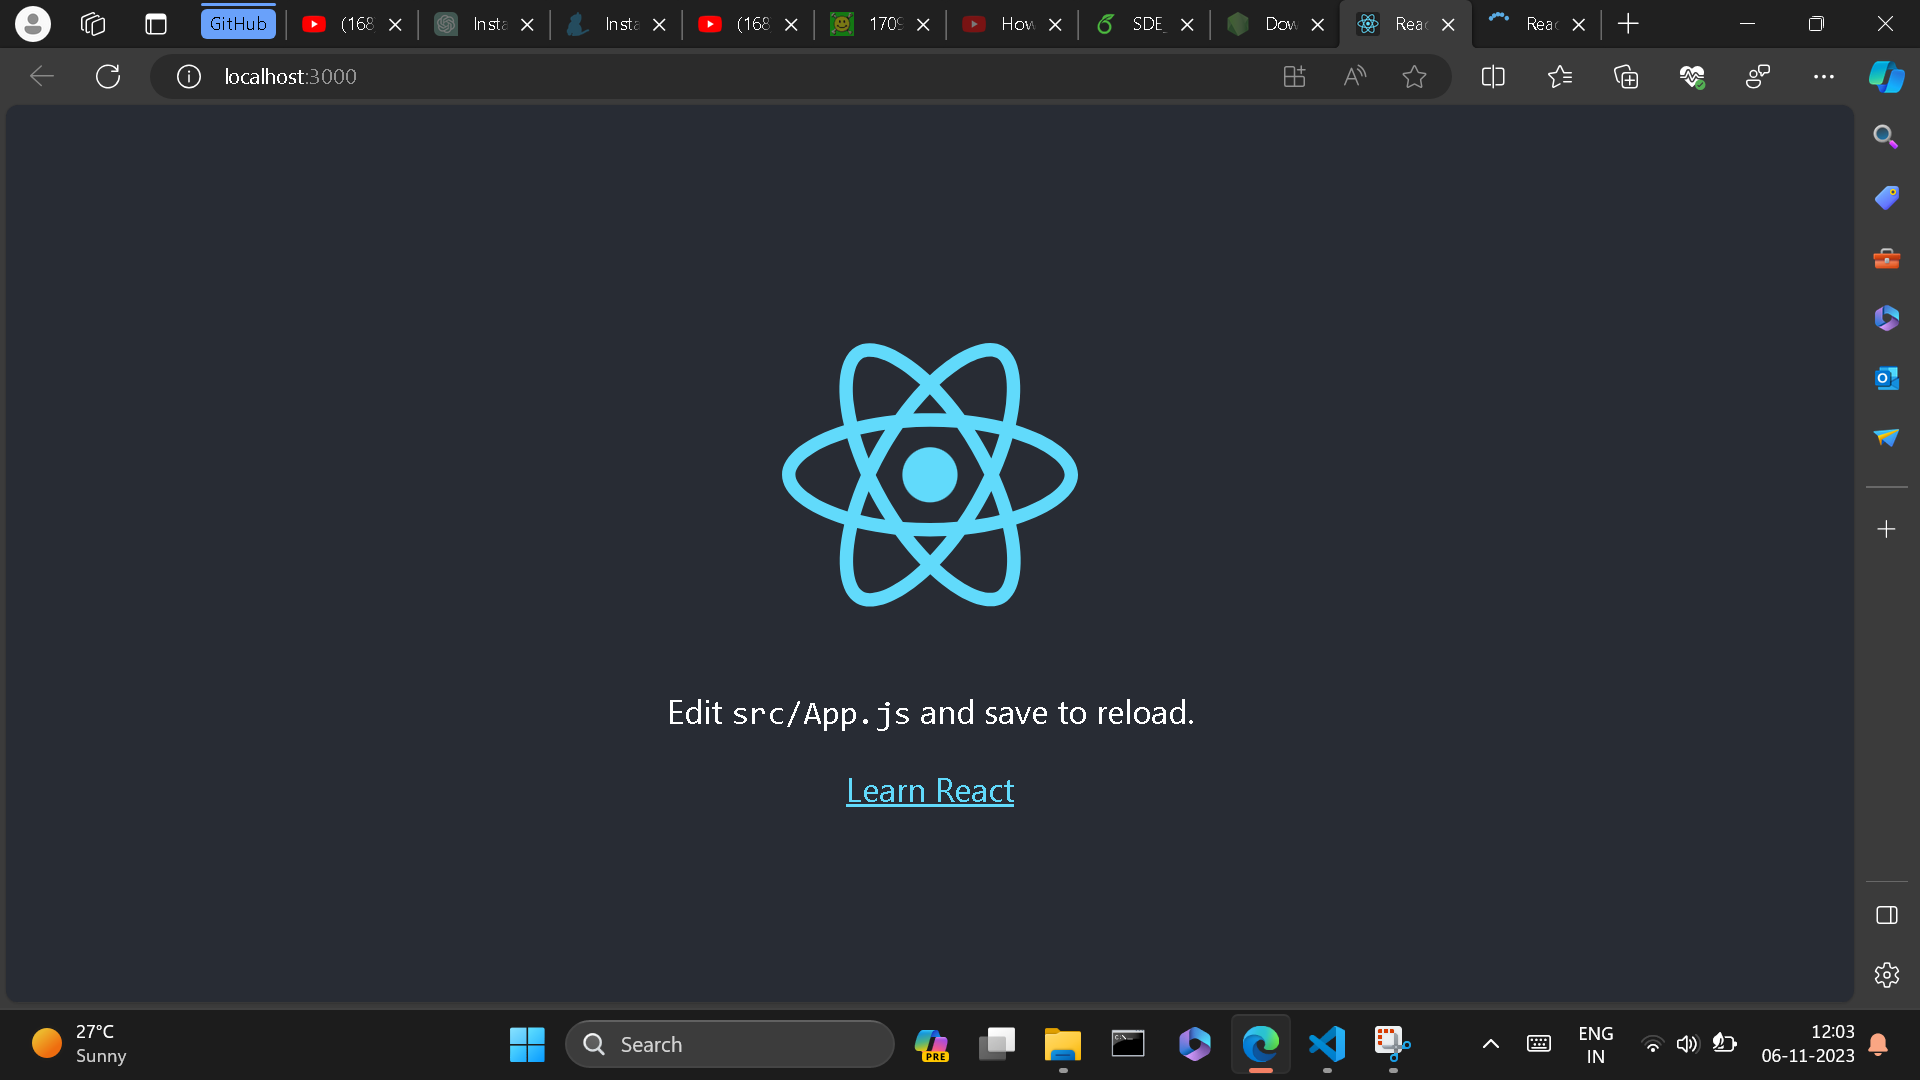
\includegraphics[width=1\textwidth]{assets/reactAppInstalled.png}
    \caption{React started}
    \label{fig:logo}
\end{figure}


\subsection{Client side routing}
Client side routing works well for small or single page websites, it helps in faster navigation through the website, as it loads the web app at once and then dynamically updates the content as per the user request.

i am using \textbf{react-router-dom} library to implement client-side routing.


\begin{listing}[htbp]
\begin{minted}[frame=single,framesep=10pt,breaklines,breakanywhere]{shell}
yarn react-router-dom
\end{minted}
\end{listing}



\begin{figure}[H]
    \centering
    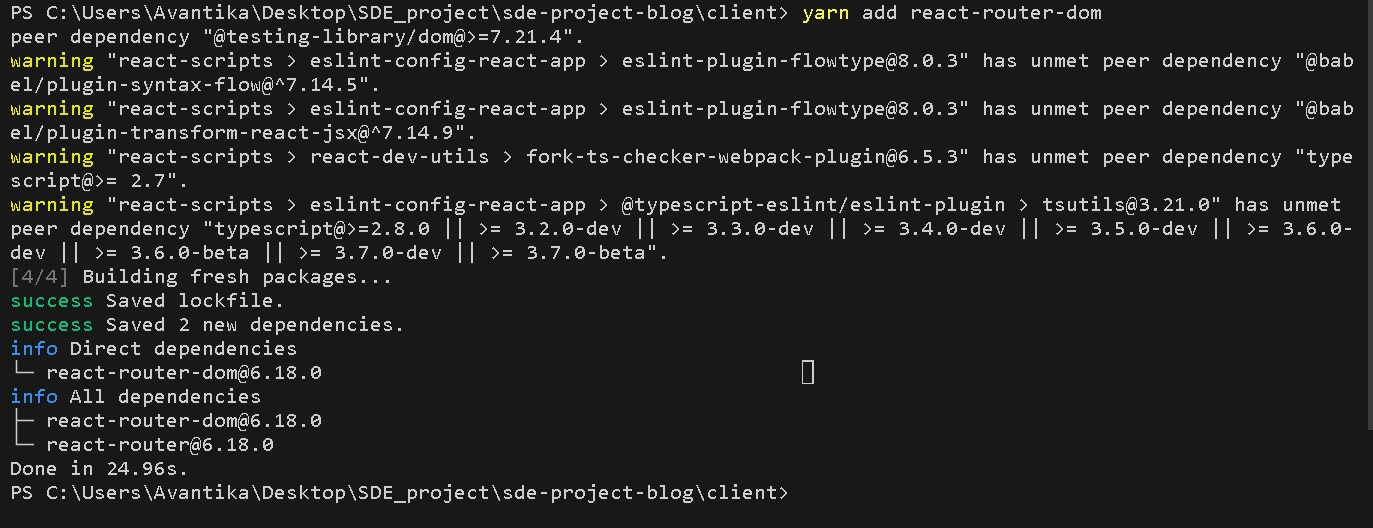
\includegraphics[width=1\textwidth]{assets/ReactRouterDom-installed.png}
    \caption{react-router-dom Installed}
    \label{fig:logo}
\end{figure}


\subsection{Installing Express}

The main app is contained in the 'client' directory and the backend APIs are managed in 'api' directory, we change the directory to 'api' and run this command to install 'Express'

\begin{listing}[htbp]
\begin{minted}[frame=single,framesep=10pt,breaklines,breakanywhere]{shell}
yarn add express
\end{minted}
\end{listing}

% \begin{listing}[H]
% \begin{minted}[frame=single,framesep=10pt,breaklines,breakanywhere]{shell}
% sudo systemctl start nginx
% sudo systemctl status nginx
% \end{minted}
% \end{listing}

\begin{figure}[H]
    \centering
    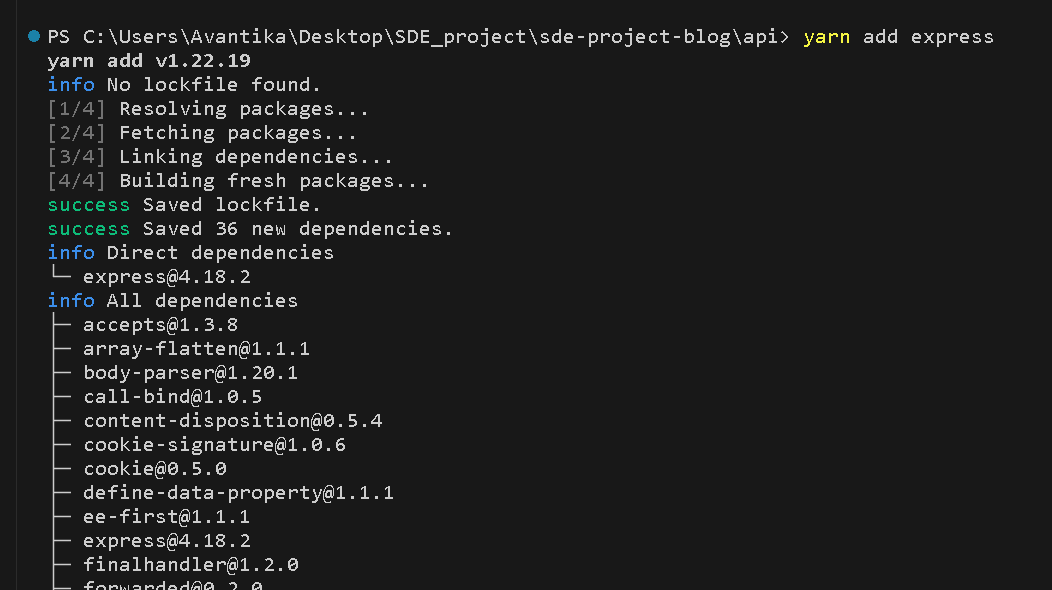
\includegraphics[width=1\textwidth]{assets/expressInstalled.png}
    \caption{Express installed in 'api' directory}
    \label{fig:logo}
\end{figure}

\subsection{Install Nodemon}

Nodemon helps to automatically restart the Node.js server (app) whenever we edit/change a file, following is the command to install 'nodemon'.

\begin{listing}[htbp]
\begin{minted}[frame=single,framesep=10pt,breaklines,breakanywhere]{shell}
yarn global add nodemon
\end{minted}
\end{listing}

\begin{figure}[H]
    \centering
    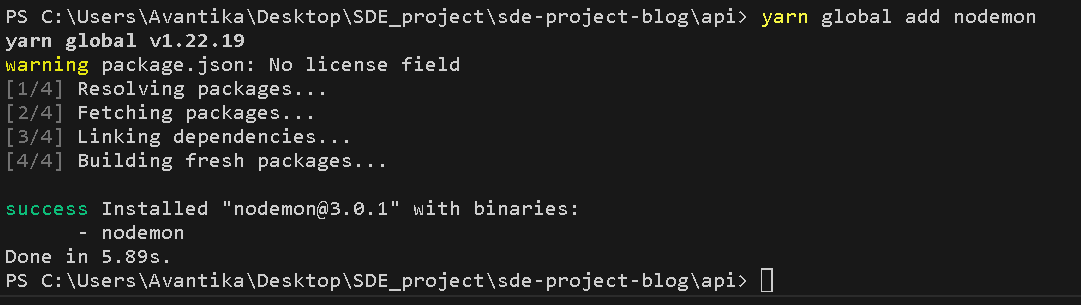
\includegraphics[width=1\textwidth]{assets/nodemonInstall.png}
    \caption{Nodemon installed}
    \label{fig:logo}
\end{figure}
\clearpage


\subsection{Installing CORS}

CORS (Cross Origin Resource Sharing) is used to prevent web pages hosted at one server to make requests at the other server, but when required this constrain can be relaxed as well.

\begin{listing}[htbp]
\begin{minted}[frame=single,framesep=10pt,breaklines,breakanywhere]{shell}
yarn add cors
\end{minted}
\end{listing}


\begin{figure}[H]
    \centering
    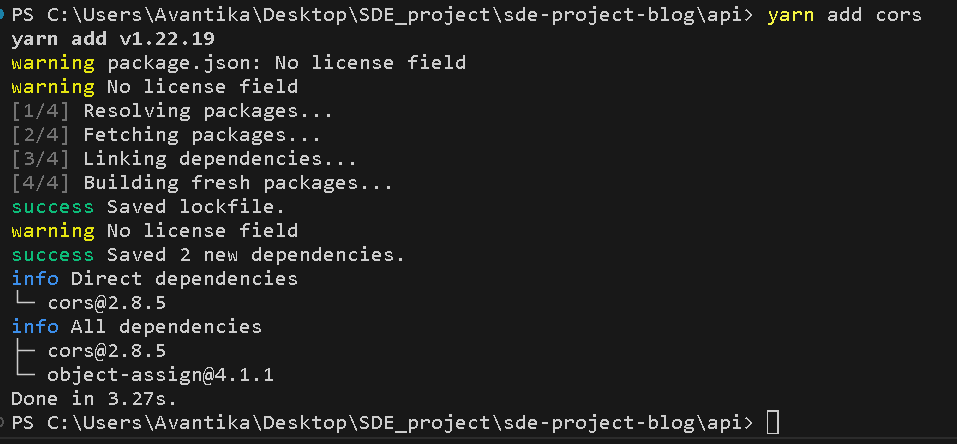
\includegraphics[width=1\textwidth]{assets/corsInstalled.png}
    \caption{Cors installed in 'api' directory}
    \label{fig:logo}
\end{figure}


\subsection{Installing JSON Web Token (JWT)}
JSON Web Token (JWT) is an open standard (RFC 7519) that defines a compact and self-contained way for securely transmitting information between parties as a JSON object. This information can be verified and trusted because it is digitally signed. 

\begin{listing}[htbp]
\begin{minted}[frame=single,framesep=10pt,breaklines,breakanywhere]{shell}
yarn add jsonwebtoken
\end{minted}
\end{listing}



\subsection{Installing cookie-parser}
 whenever a user visits the website, and their browser sends cookies, the app uses cookie-parser to automatically understand and organize those cookies. 
 
\begin{listing}[htbp]
\begin{minted}[frame=single,framesep=10pt,breaklines,breakanywhere]{shell}
yarn add cookie-parser
\end{minted}
\end{listing}

\clearpage

\subsection{react-quill}

React Quill is a text editor that will be used to edit or write posts in the web-app as well as format the text on the web page itself.

\begin{listing}[htbp]
\begin{minted}[frame=single,framesep=10pt,breaklines,breakanywhere]{shell}
yarn add react-quill
\end{minted}
\end{listing}


\subsection{Multer library}

Multer library is used to for handling file uploads in Express and Node
 
\begin{listing}[htbp]
\begin{minted}[frame=single,framesep=10pt,breaklines,breakanywhere]{shell}
yarn add multer
\end{minted}
\end{listing}



\subsection{date-fns}

This library is used to deal with dates in JavaScript, it will be used to display the date when a post is published
 
\begin{listing}[htbp]
\begin{minted}[frame=single,framesep=10pt,breaklines,breakanywhere]{shell}
yarn add date-fns
\end{minted}
\end{listing}



\subsection{dotenv}

Dotenv is used to load environment variables from a .env file. This is useful for storing configuration settings and sensitive information (MongoDB connection string with password) without hardcoding them in your code.


\subsection{connect-mongo \& express-session}

express-session is used for session management and connect-mongo is used along with it to store the user session data in MongoDB database instead of server memory this is used to prevent data loss in case of server restart

\begin{listing}[H]
\begin{minted}[frame=single,framesep=10pt,breaklines,breakanywhere]{shell}
npm i connect-mongo
npm i express-session
\end{minted}
\end{listing}


\clearpage


\section{Task 2: Setting up MongoDB database}

\begin{figure}[H]
    \centering
    \includegraphics[width=1\textwidth]{assets/MongoDB_Fores-Green.svg.png}
    \caption{MongoDB}
    \label{fig:logo}
\end{figure}


\subsection{Setting up Mongo DB}

Monog DB is a database that we will be using for storing the various user information such as username and passwords in it, as weel as the posts
To set up MongoDB, we need to first go to the official website of MongoDB and create a 'New Project' by clicking on the button at top right corner.


\begin{figure}[H]
    \centering
    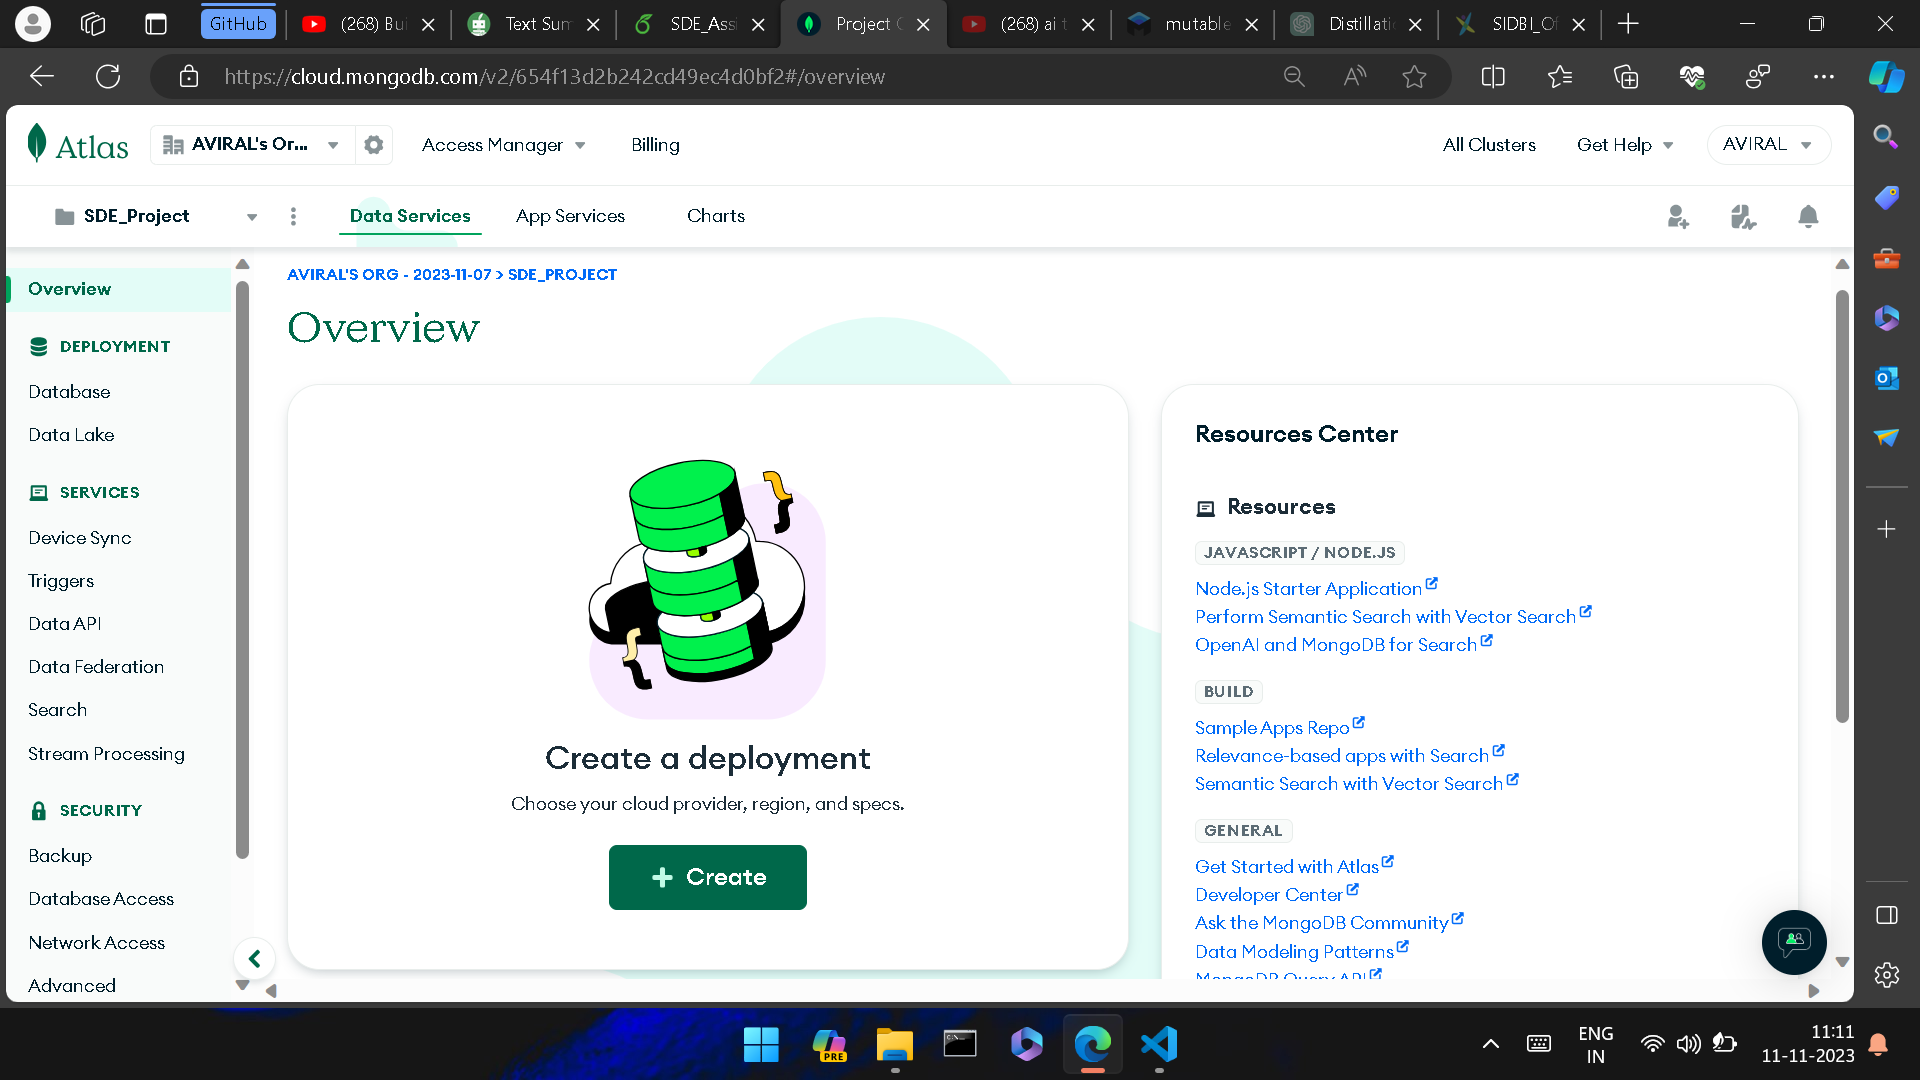
\includegraphics[width=1\textwidth]{assets/creatingMongoDB-database.png}
    \caption{MongoDB New project (SDE\_Node\_JS\_Blog) created}
    \label{fig:logo}
\end{figure}

click on "create" button to create a new cluster, and follow the required steps. Then to connect with the code we need to install mongose

\begin{figure}[H]
    \centering
    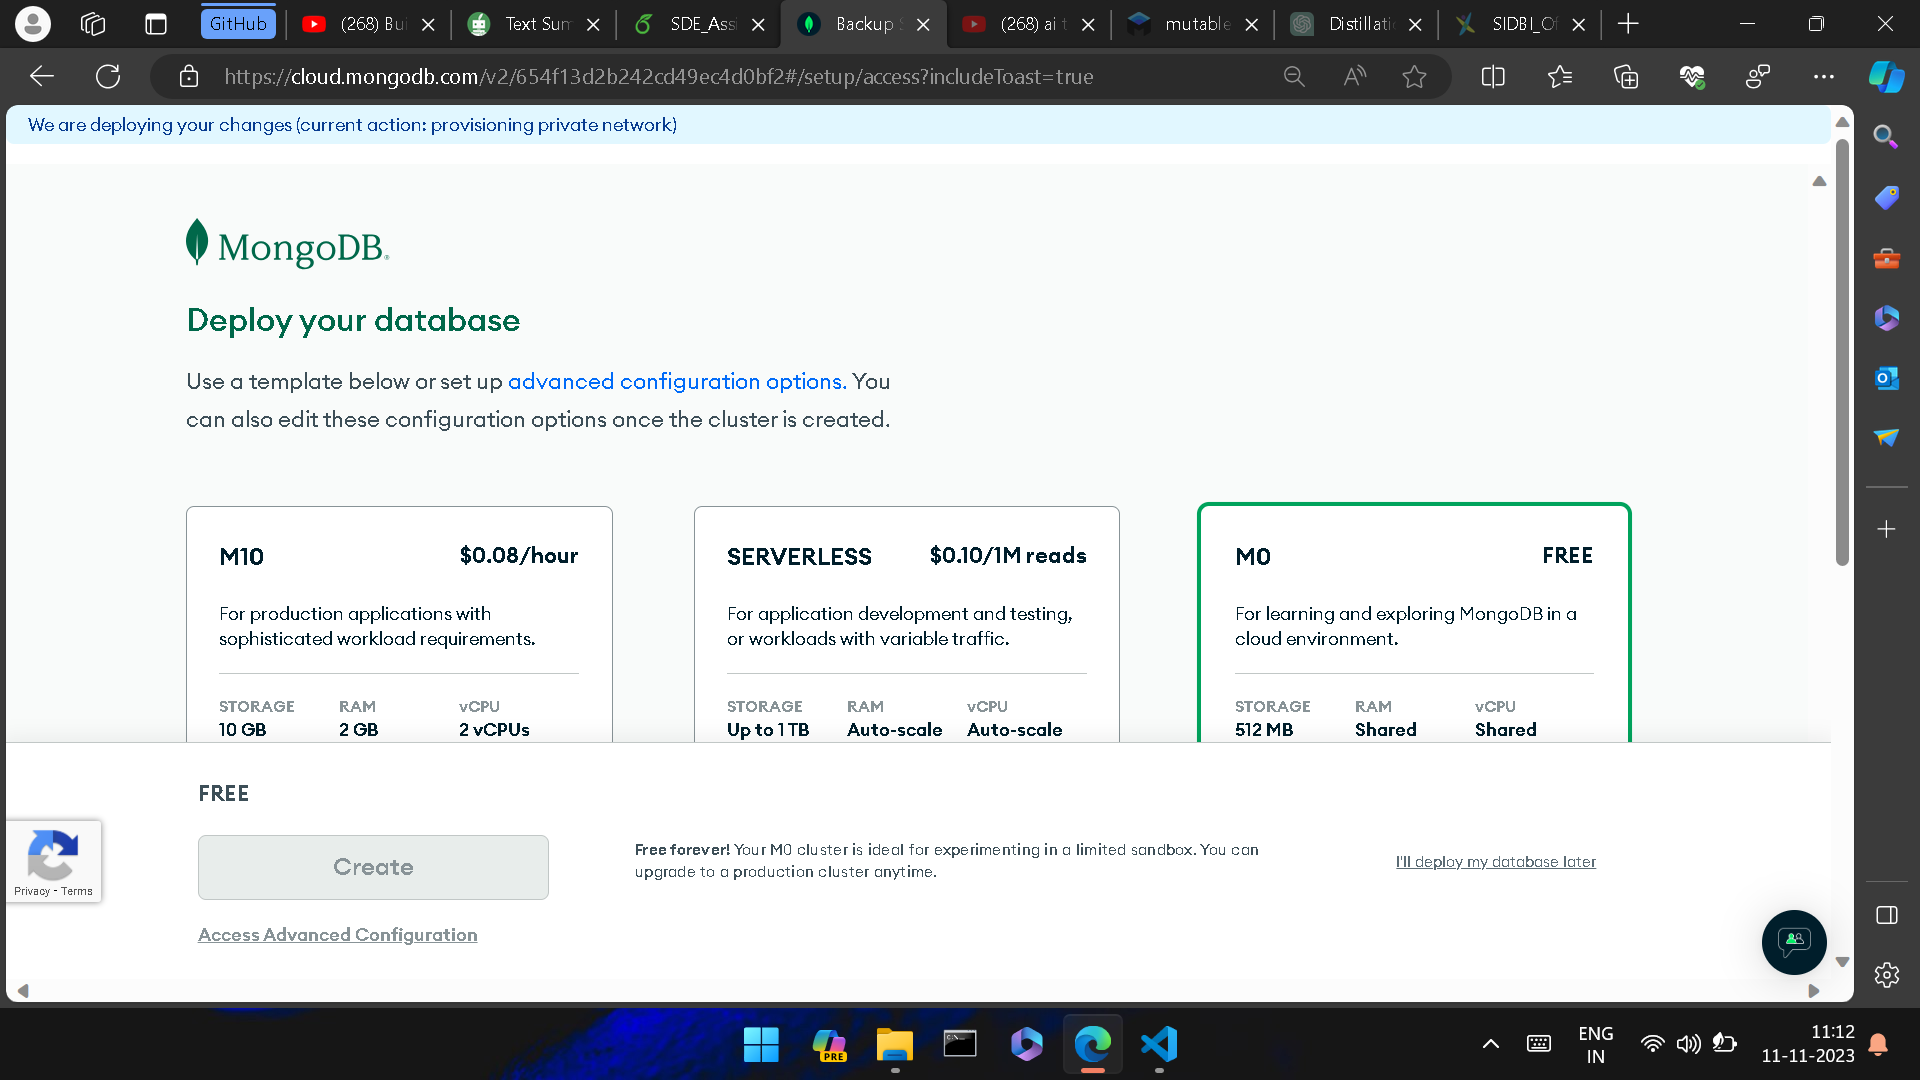
\includegraphics[width=1\textwidth]{assets/MongoDB-Deployment.png}
    \caption{MongoDB Deployment using 'free' version}
    \label{fig:logo}
\end{figure}

\begin{figure}[H]
    \centering
    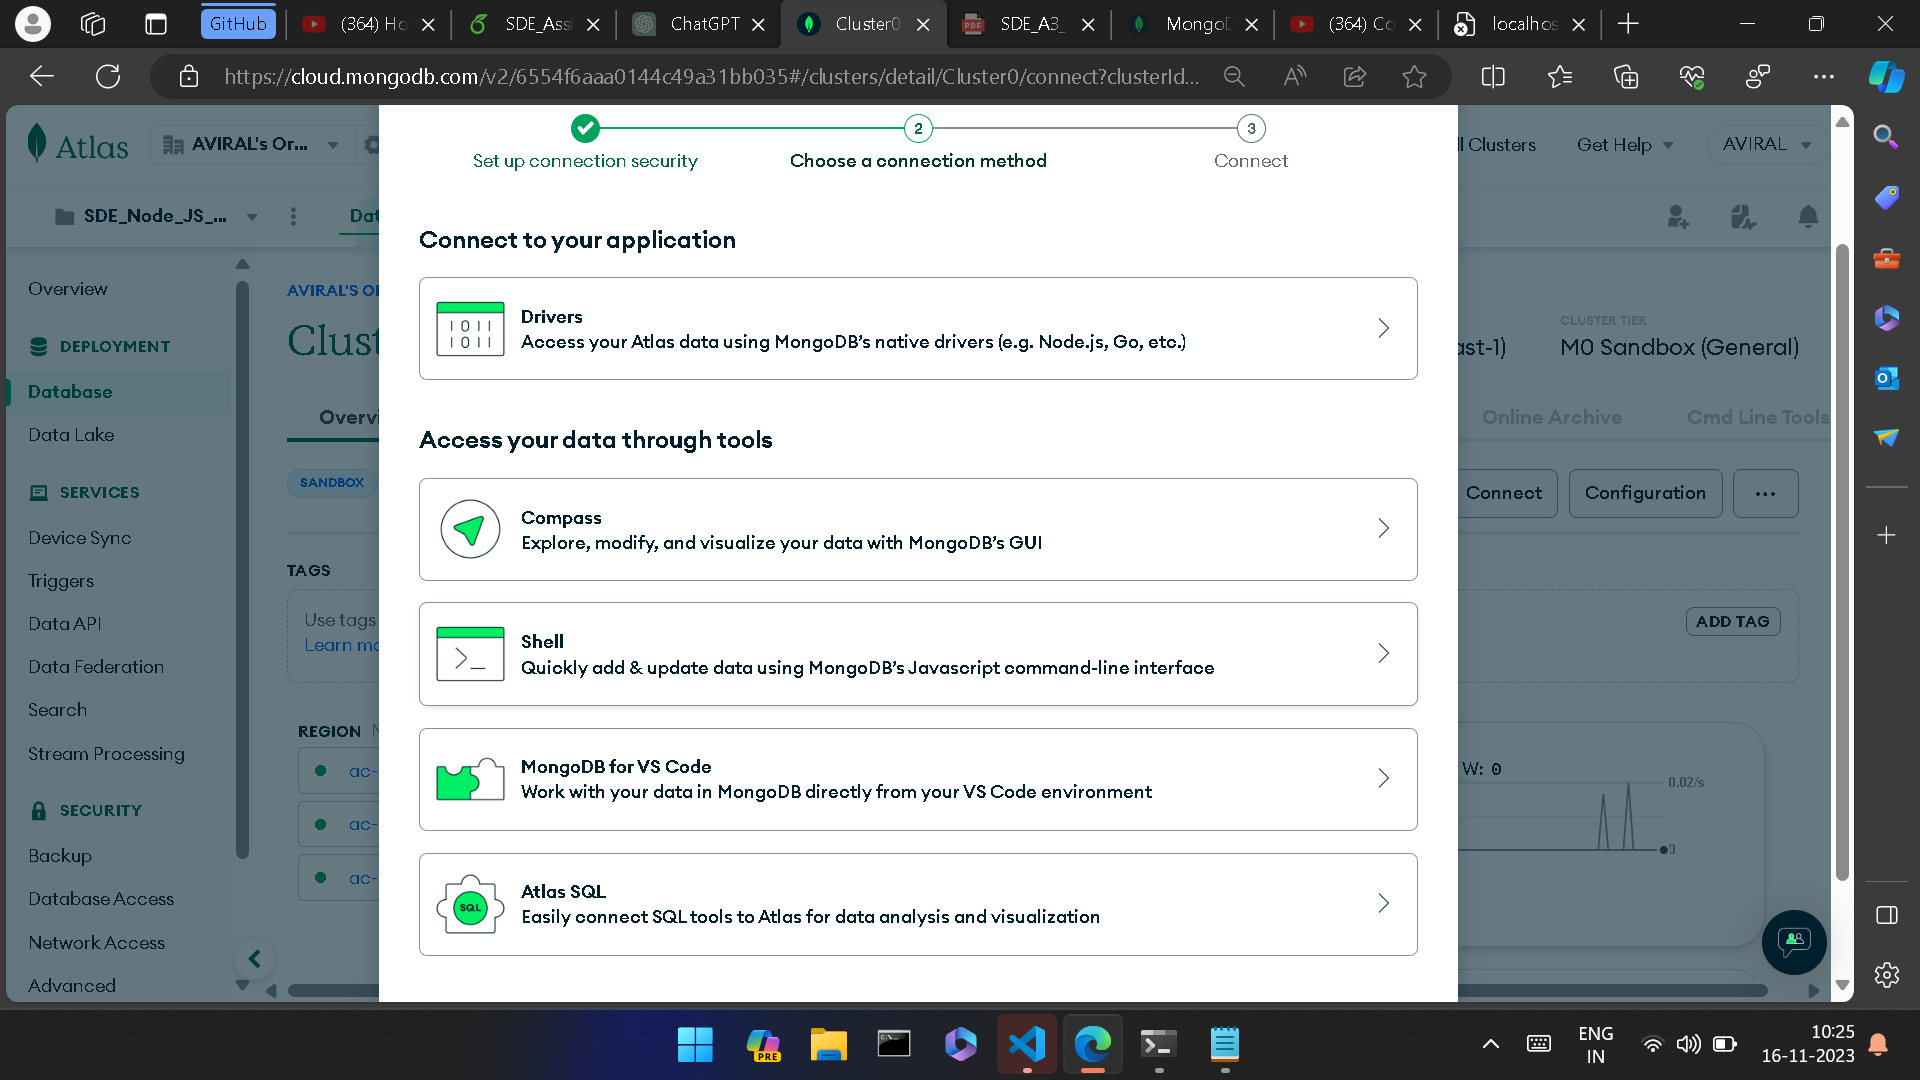
\includegraphics[width=1\textwidth]{assets/mongoDB_VScode_connect.png}
    \caption{connecting MongoDB to VS Code}
    \label{fig:logo}
\end{figure}

\clearpage

\begin{figure}[H]
    \centering
    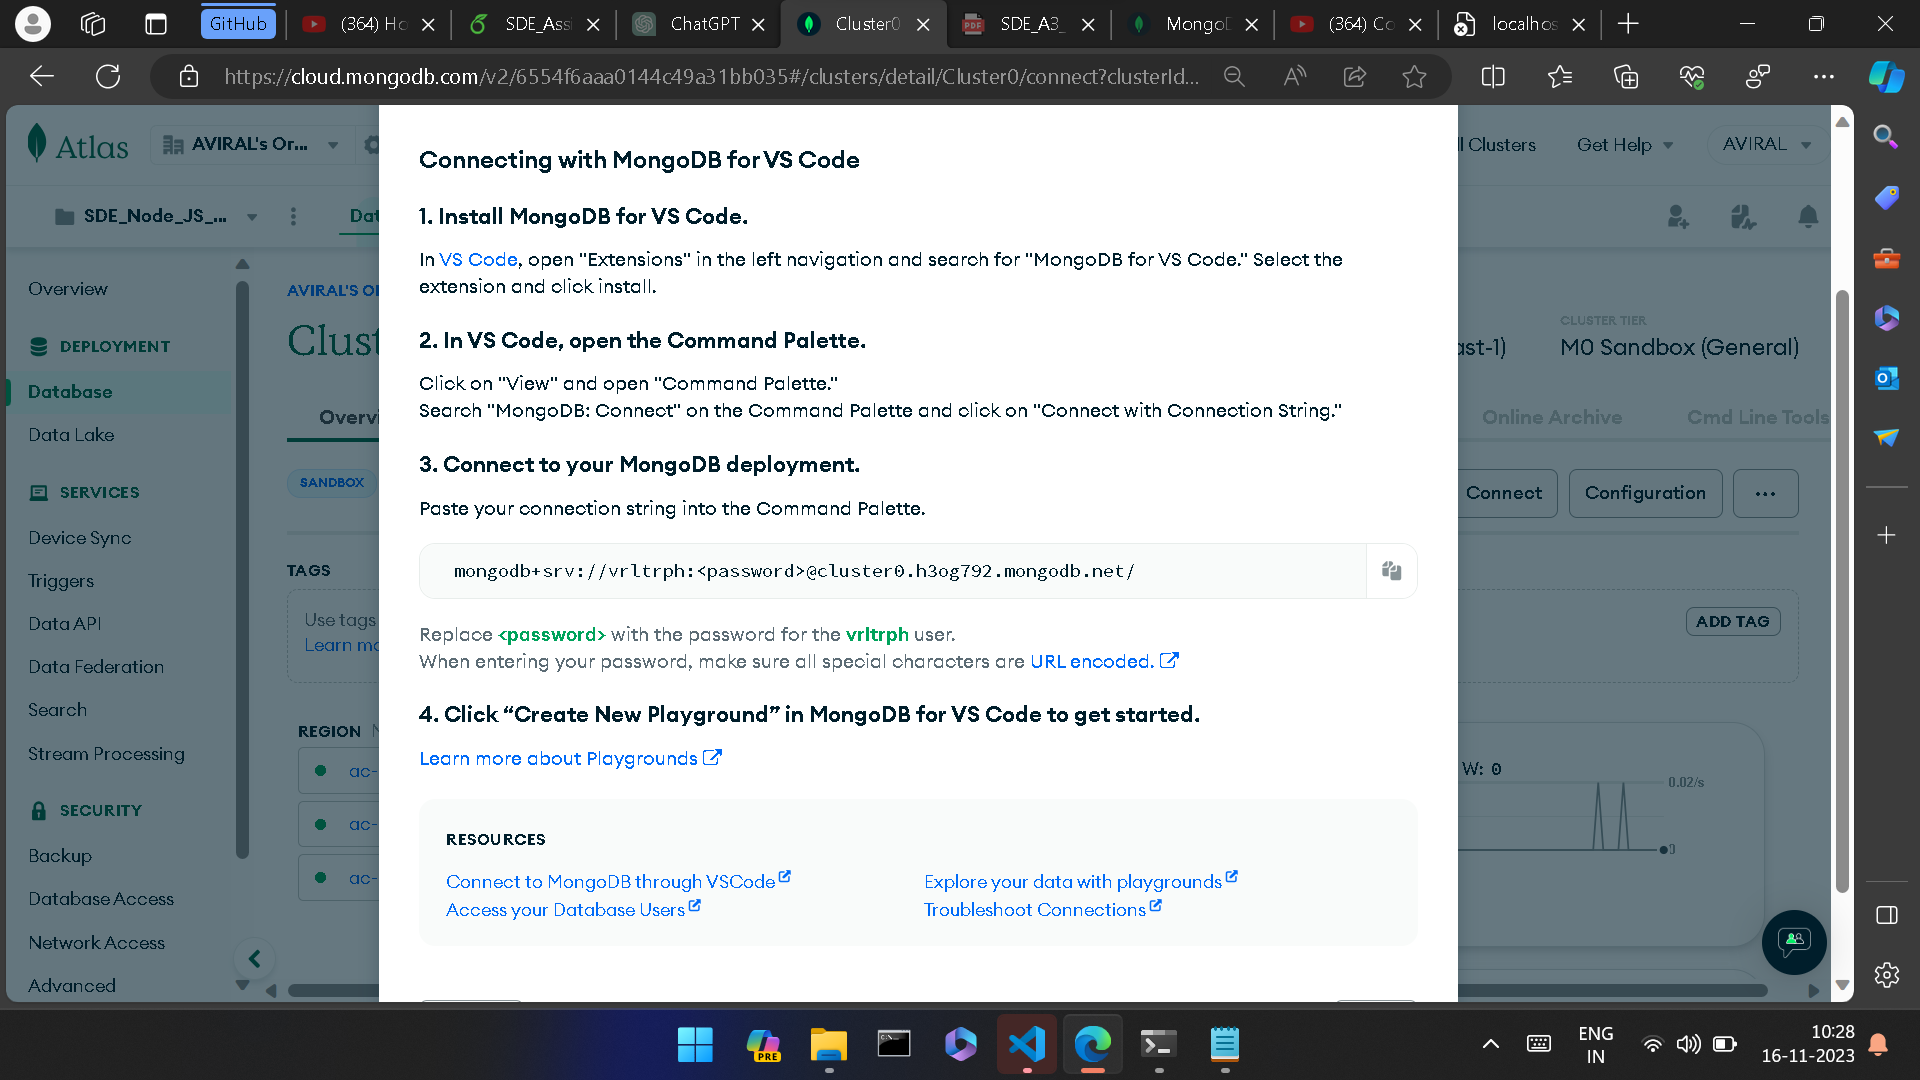
\includegraphics[width=1\textwidth]{assets/VScode_MongoDB_connect.png}
    \caption{Copy the connection string and put it in .env file in VS Code}
    \label{fig:logo}
\end{figure}


\begin{listing}[htbp]
\begin{minted}[frame=single,framesep=10pt,breaklines,breakanywhere]{shell}
yarn add mongose
\end{minted}
\end{listing}


\begin{figure}[H]
    \centering
    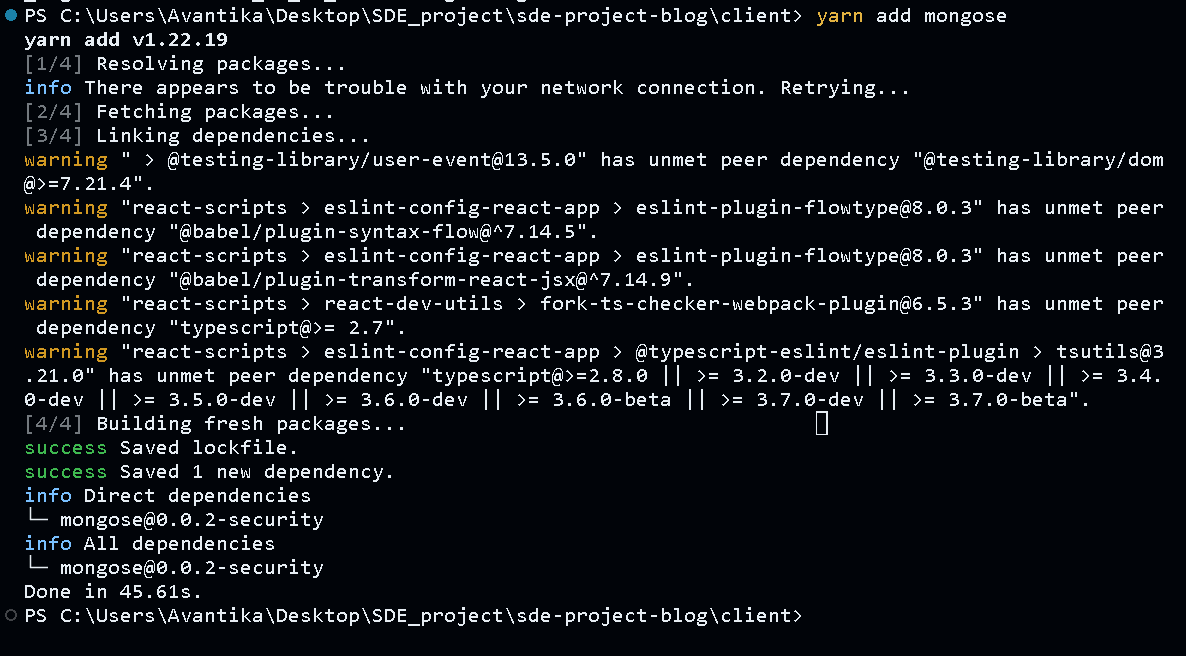
\includegraphics[width=1\textwidth]{assets/MongoseDBinsatllationCommand.png}
    \caption{MongoDB installed on our computer}
    \label{fig:logo}
\end{figure}



\begin{figure}[H]
    \centering
    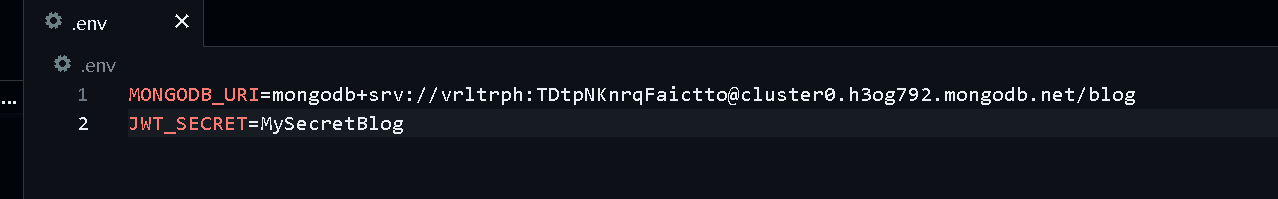
\includegraphics[width=1\textwidth]{assets/dotenv_file.png}
    \caption{.env file in VS Code}
    \label{fig:logo}
\end{figure}

This code is then used to connect with the database:

\begin{listing}[htbp]
\begin{minted}[frame=single,framesep=10pt,breaklines,breakanywhere]{shell}
const mongoose = require('mongoose');
const connectDB = async () => {
  
  try {
    mongoose.set('strictQuery', false);
    const conn = await mongoose.connect(process.env.MONGODB_URI);
    console.log(`Database Connected: ${conn.connection.host}`);
  } catch (error) {
    console.log(error);
  }

}

module.exports = connectDB;

\end{minted}
\end{listing}


once we are connected to MongoDB, we will see the data in it in the 'collections' tab:

\begin{figure}[H]
    \centering
    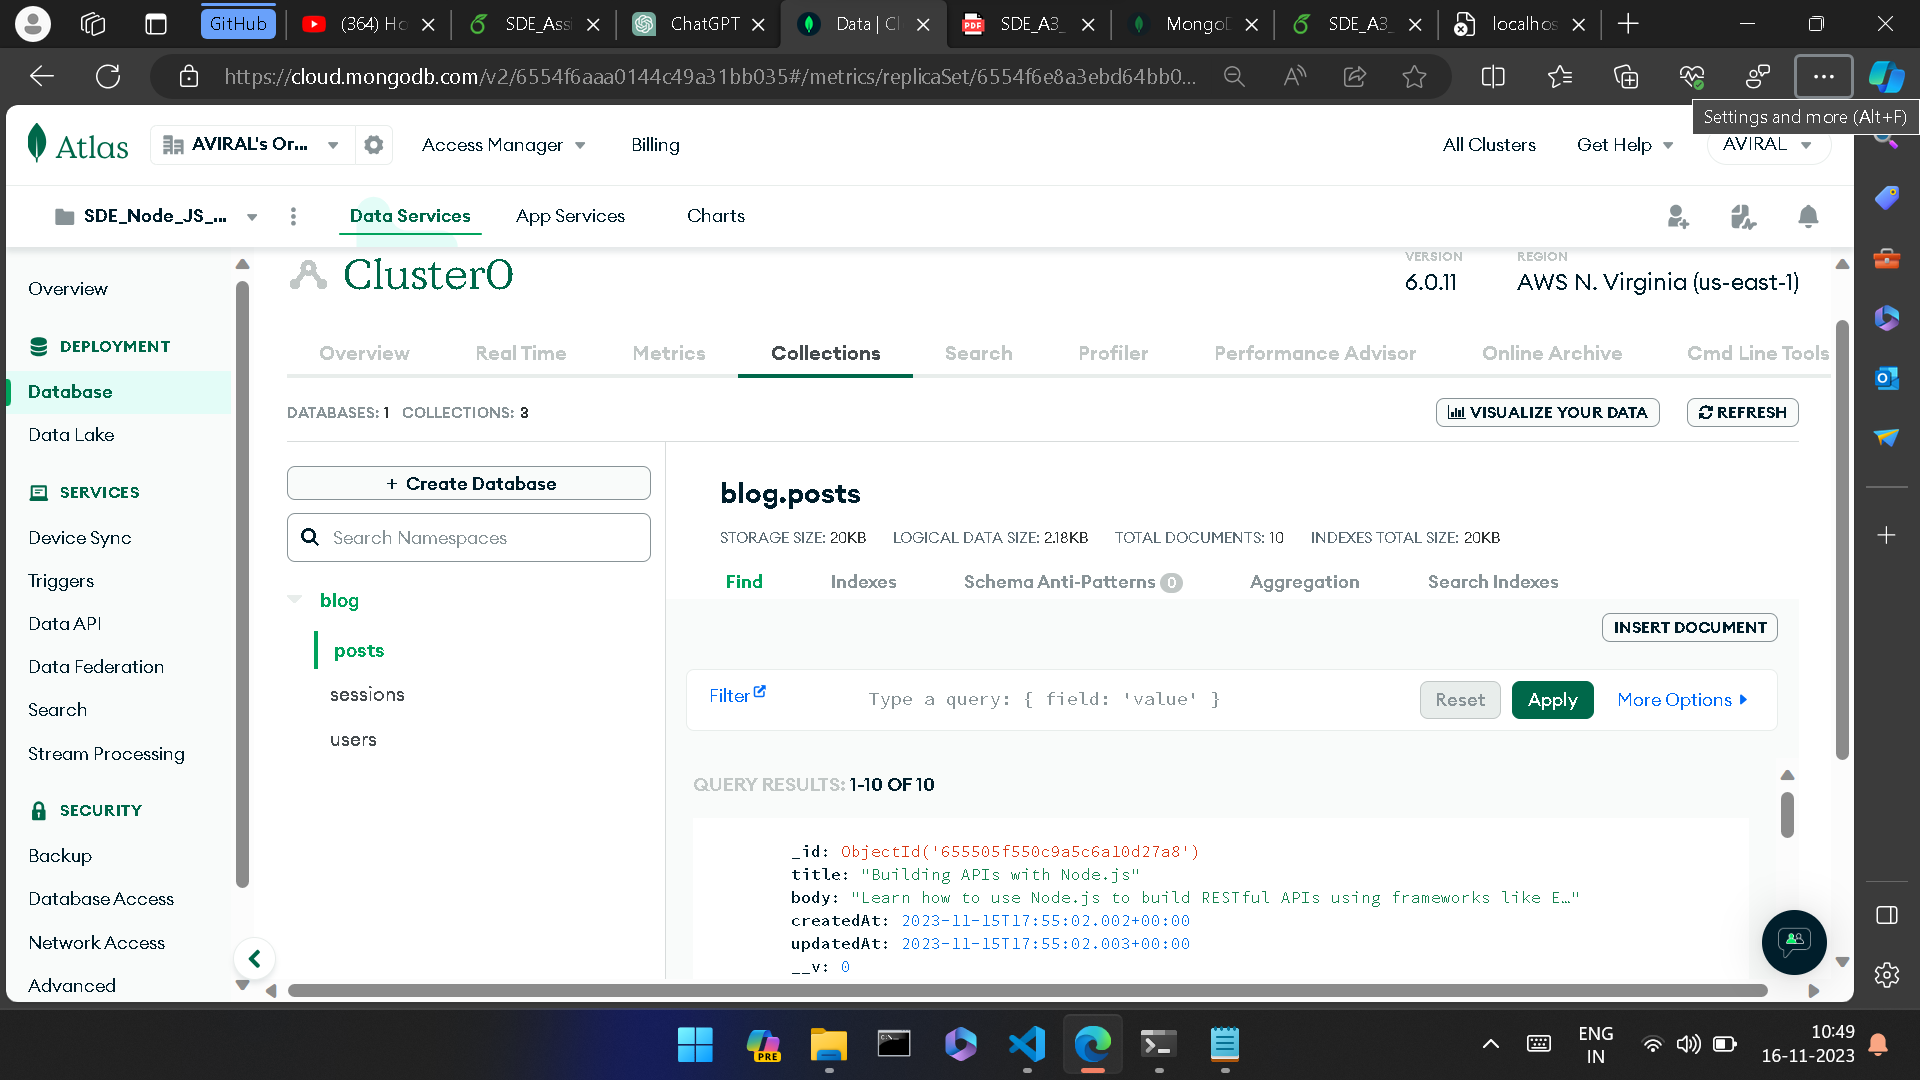
\includegraphics[width=1\textwidth]{assets/mongoDB_collections.png}
    \caption{MongoDB Collections}
    \label{fig:logo}
\end{figure}


\subsection{Installing bcryptjs}

In the database the passwords are directly exposed to anyone who has an access to the database, we use bcryptjs to encrypt (hash) the passwords, so they are no seen as plane text or strings.

\begin{listing}[htbp]
\begin{minted}[frame=single,framesep=10pt,breaklines,breakanywhere]{shell}
yarn add bycryptjs
\end{minted}
\end{listing}


\begin{figure}[H]
    \centering
    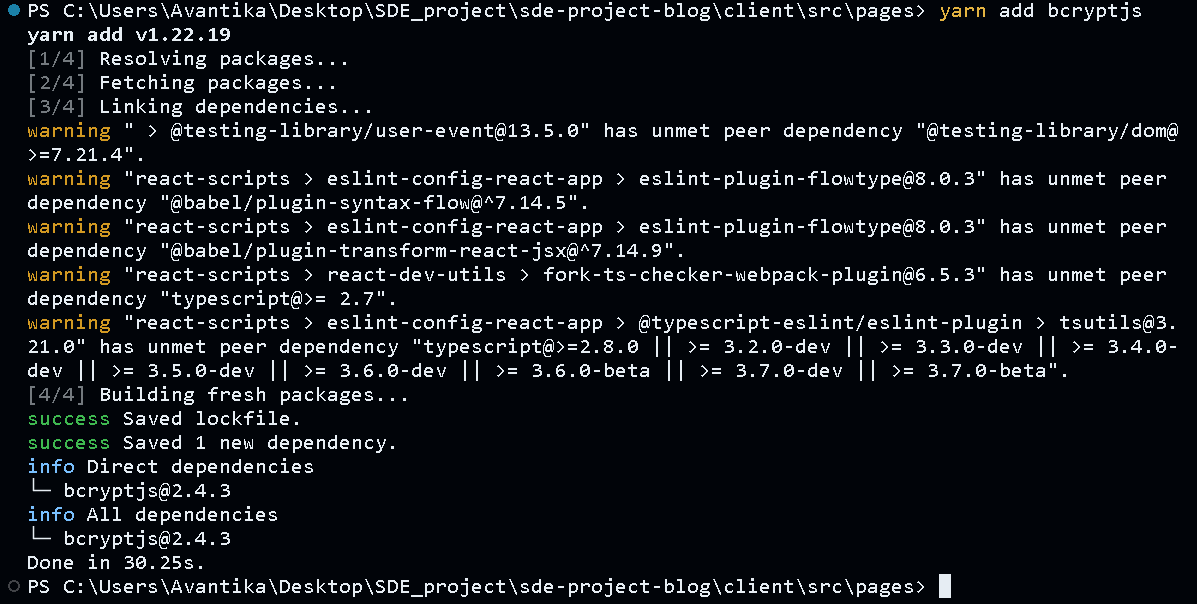
\includegraphics[width=1\textwidth]{assets/bycryptjs-installation.png}
    \caption{Bycryptjs installation}
    \label{fig:logo}
\end{figure}



% having done this, we need to copy the command for connecting to the database, and paste it into the code.

% \begin{figure}[H]
%     \centering
%     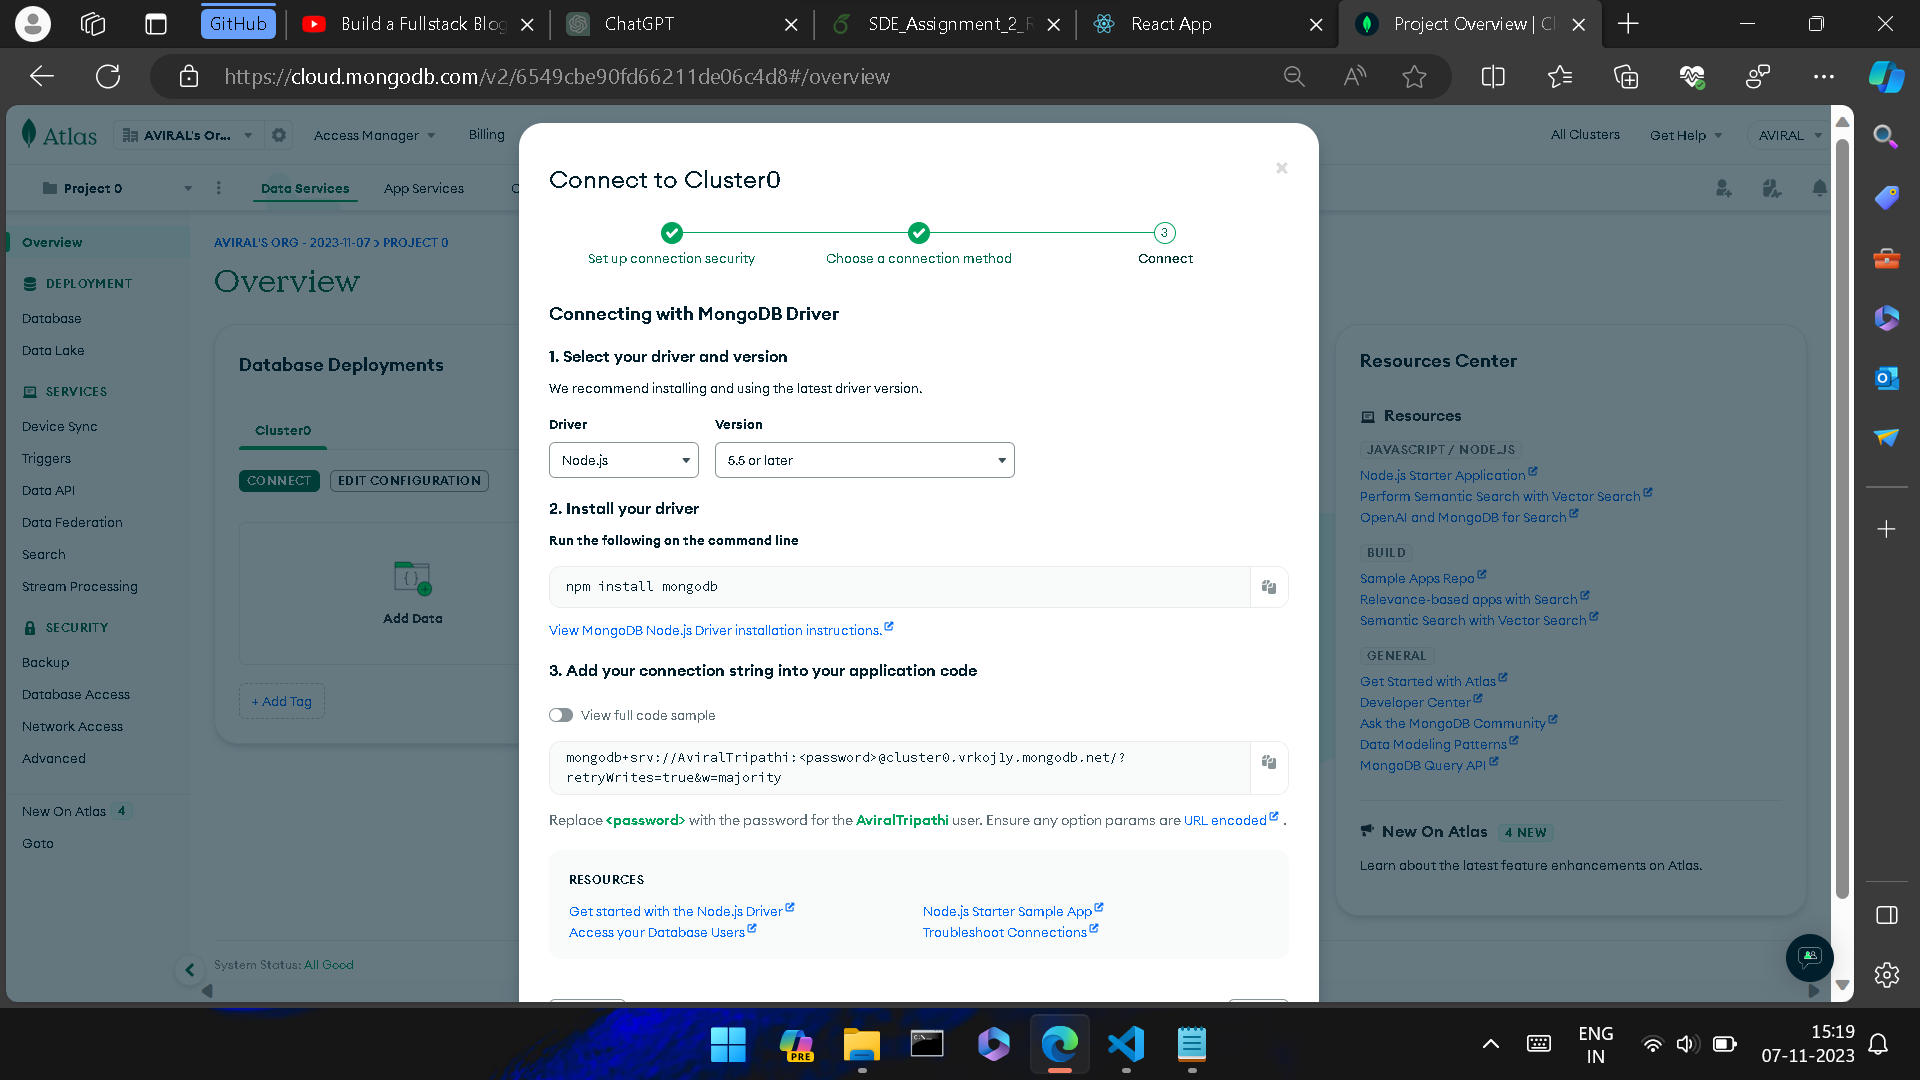
\includegraphics[width=1\textwidth]{assets/mongoDB-installation.png}
%     \caption{Connecting to MongoDB}
%     \label{fig:logo}
% \end{figure}

\clearpage

\clearpage


\section{Final Results}
After all the front-end and back-end implementation our MERN blog is ready to use, and have the following features:

\begin{itemize}[noitemsep]
  \itemsep0.5em
  
  \item A user can Register with unique 'username' and 'password'.
  \item A user can login with previously registered username and password.
  \item A Registered user can 'create', 'edit', and 'delete' the posts in the blog.
  \item All the data such as: usernames, passwords, post contents, and a user's session data is stored in Mongo DB database.

\end{itemize}

\subsection{Starting the App}
To start the app we just need to navigate to the project directory in PowerShell and type: \textbf{\textit{npm run dev}}, this command will run the 'dev' script for the project present in packages.json file

\begin{figure}[H]
    \centering
    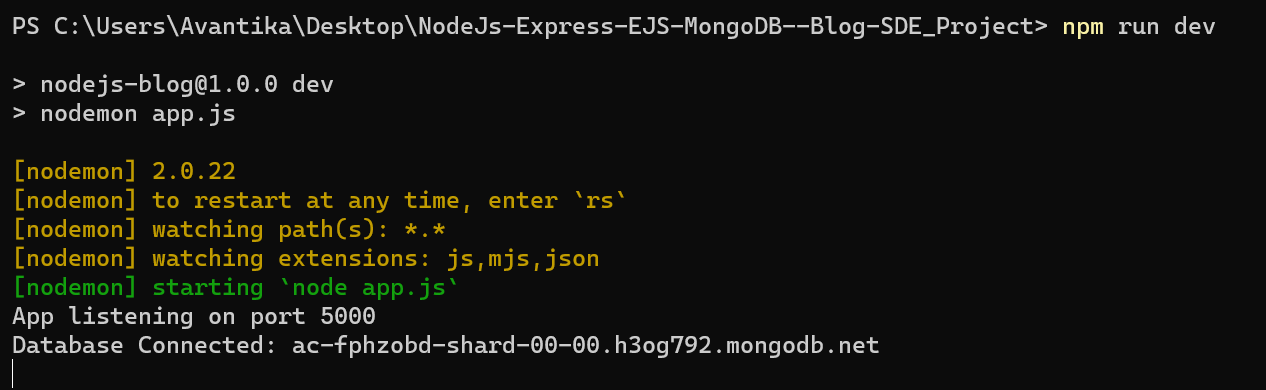
\includegraphics[width=1\textwidth]{assets/startingTheApp.png}
    \caption{Starting the MERN blog app}
    \label{fig:logo}
\end{figure}

As the app is runing on port 5000 (by default),we go to the browser and type 'localhost:5000' and press enter to display the homepage of the blog

\begin{figure}[H]
    \centering
    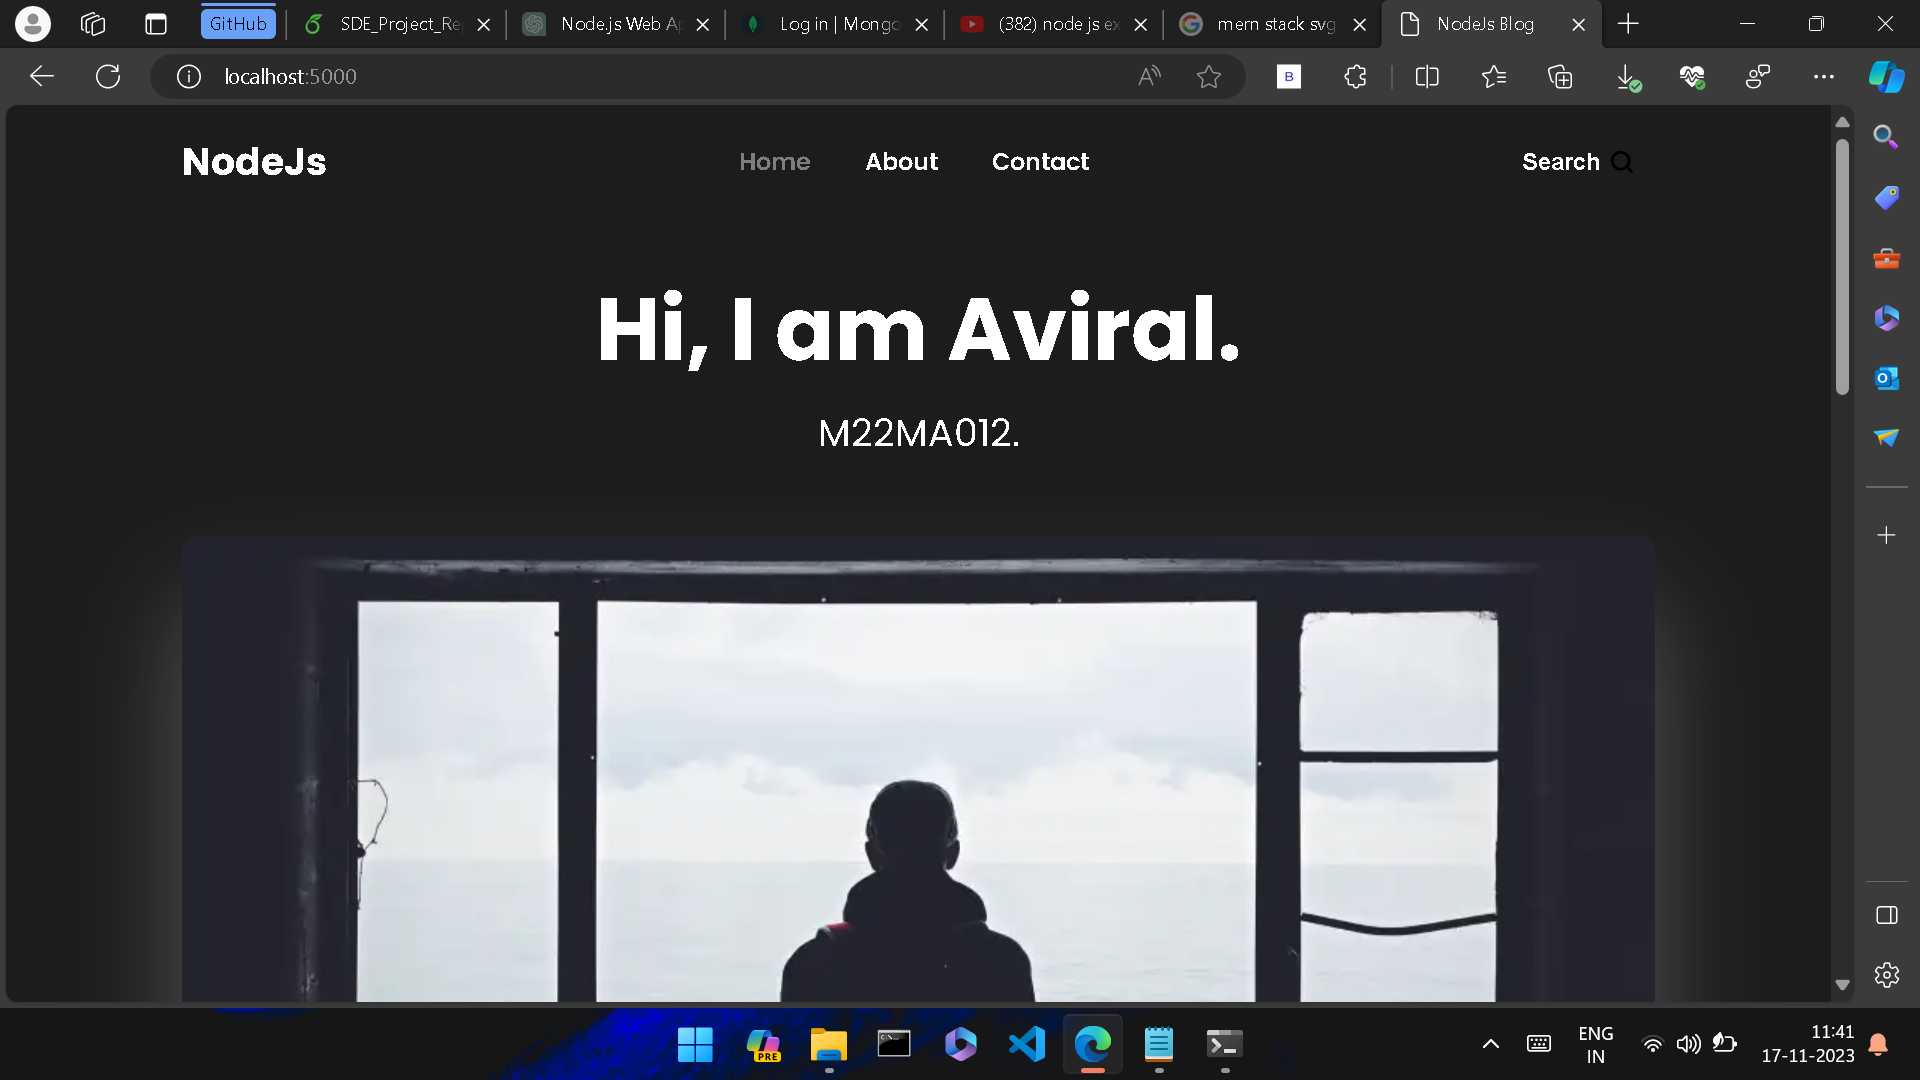
\includegraphics[width=1\textwidth]{assets/HomePage.png}
    \caption{Homepage of the MERN blog app}
    \label{fig:logo}
\end{figure}

Scrolling further down we can see the posts in the blog

\begin{figure}[H]
    \centering
    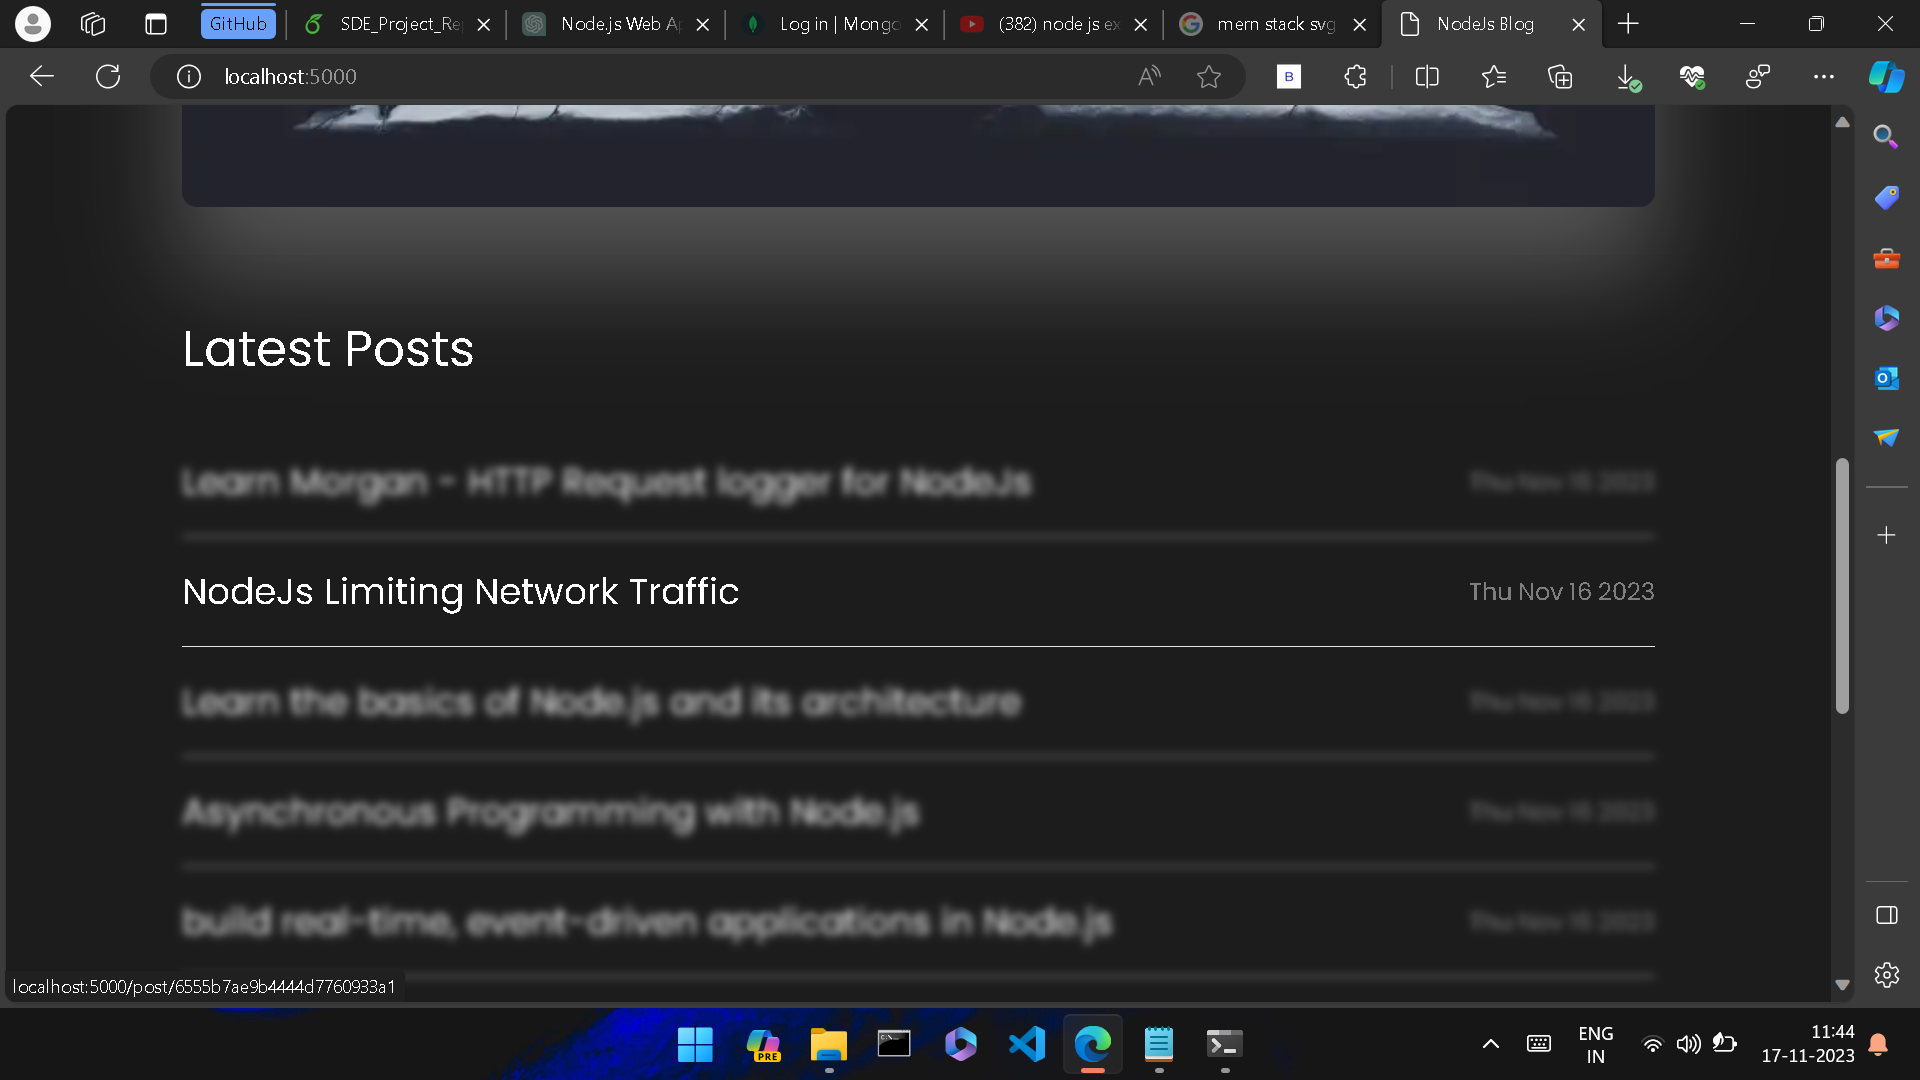
\includegraphics[width=1\textwidth]{assets/homepagePosts.png}
    \caption{Homepage Posts}
    \label{fig:logo}
\end{figure}

\clearpage

It can be verified that these posts are stored in the MongoDB (Atlas) database, and can be seen there:

\begin{figure}[H]
    \centering
    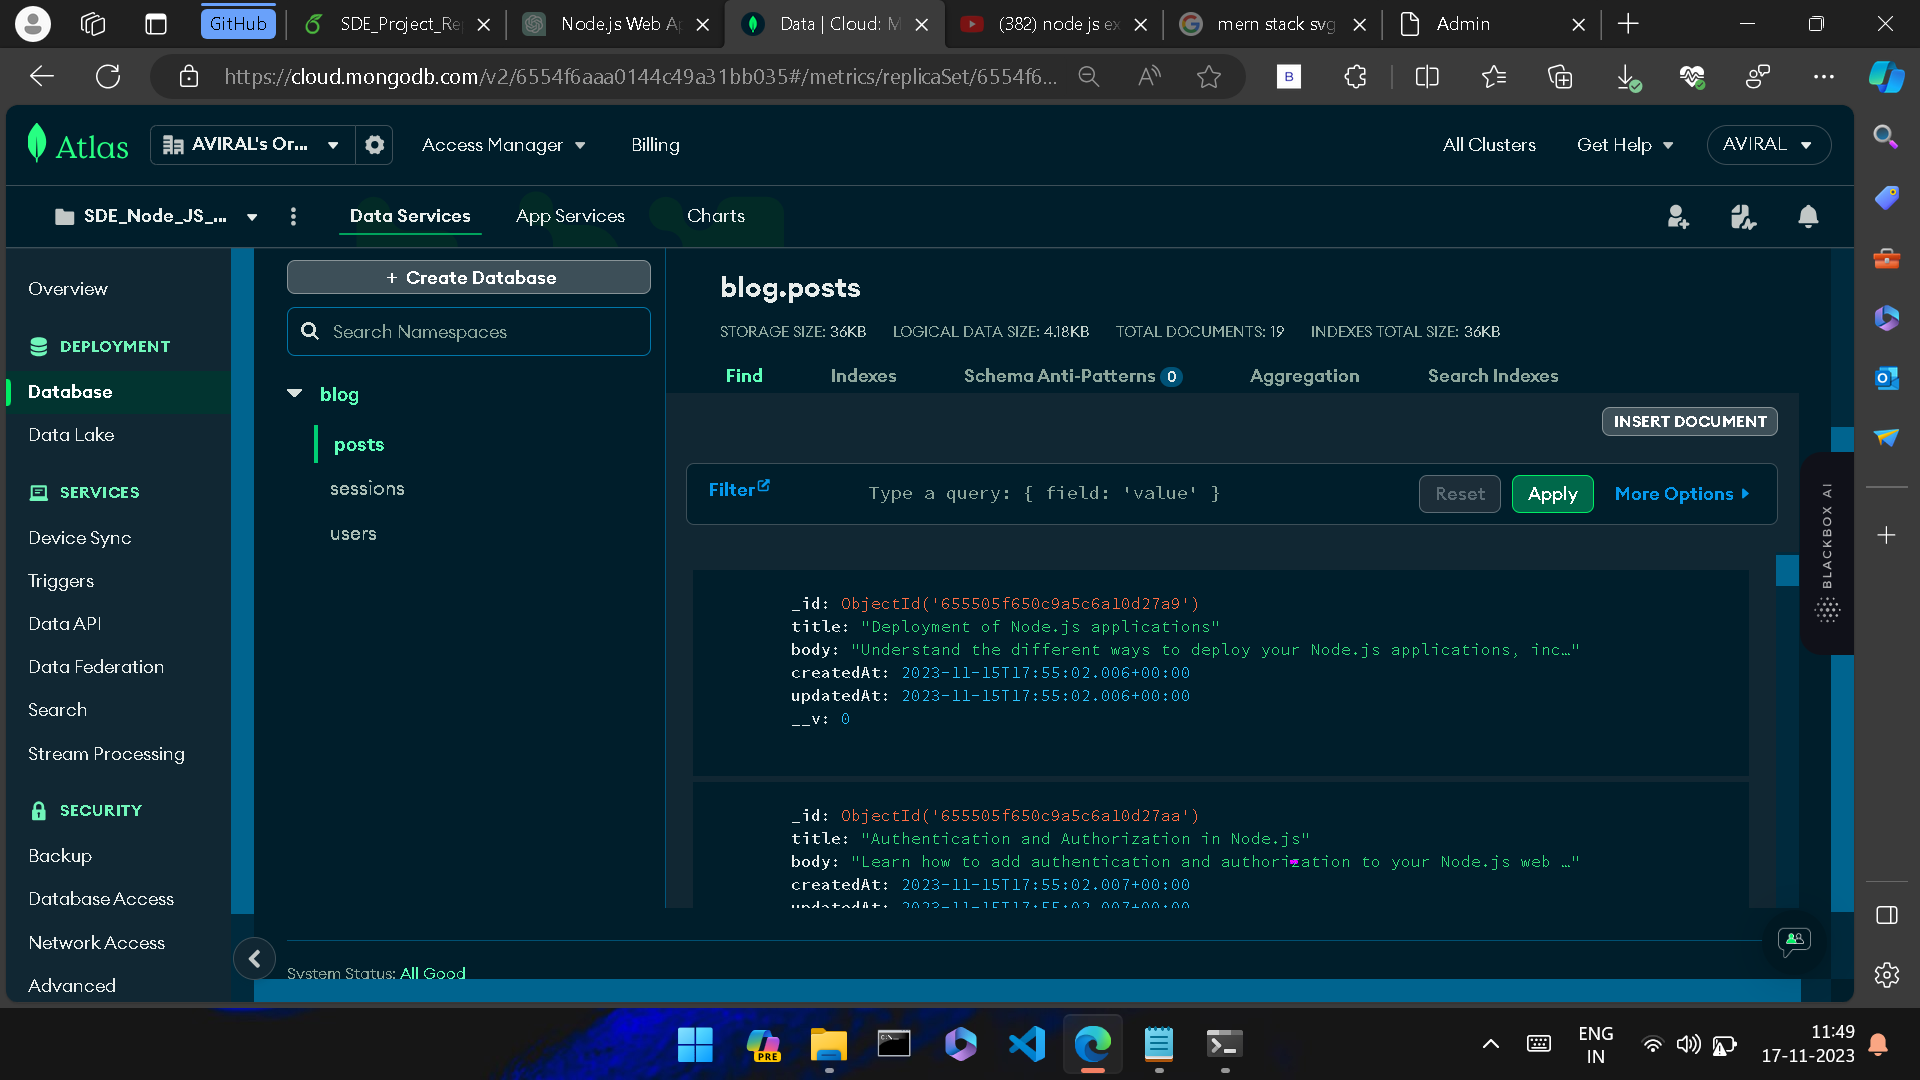
\includegraphics[width=1\textwidth]{assets/PostsInMongoDB.png}
    \caption{Posts in MongoDB (Atlas)}
    \label{fig:logo}
\end{figure}

Upon visitng 'localhost:5000/admin' in the browser tab we can see the login and regestration forms, if we register a user, we can find its username and password (Hashed by bcrypt) in MongoDB (Atlas)

\begin{figure}[H]
    \centering
    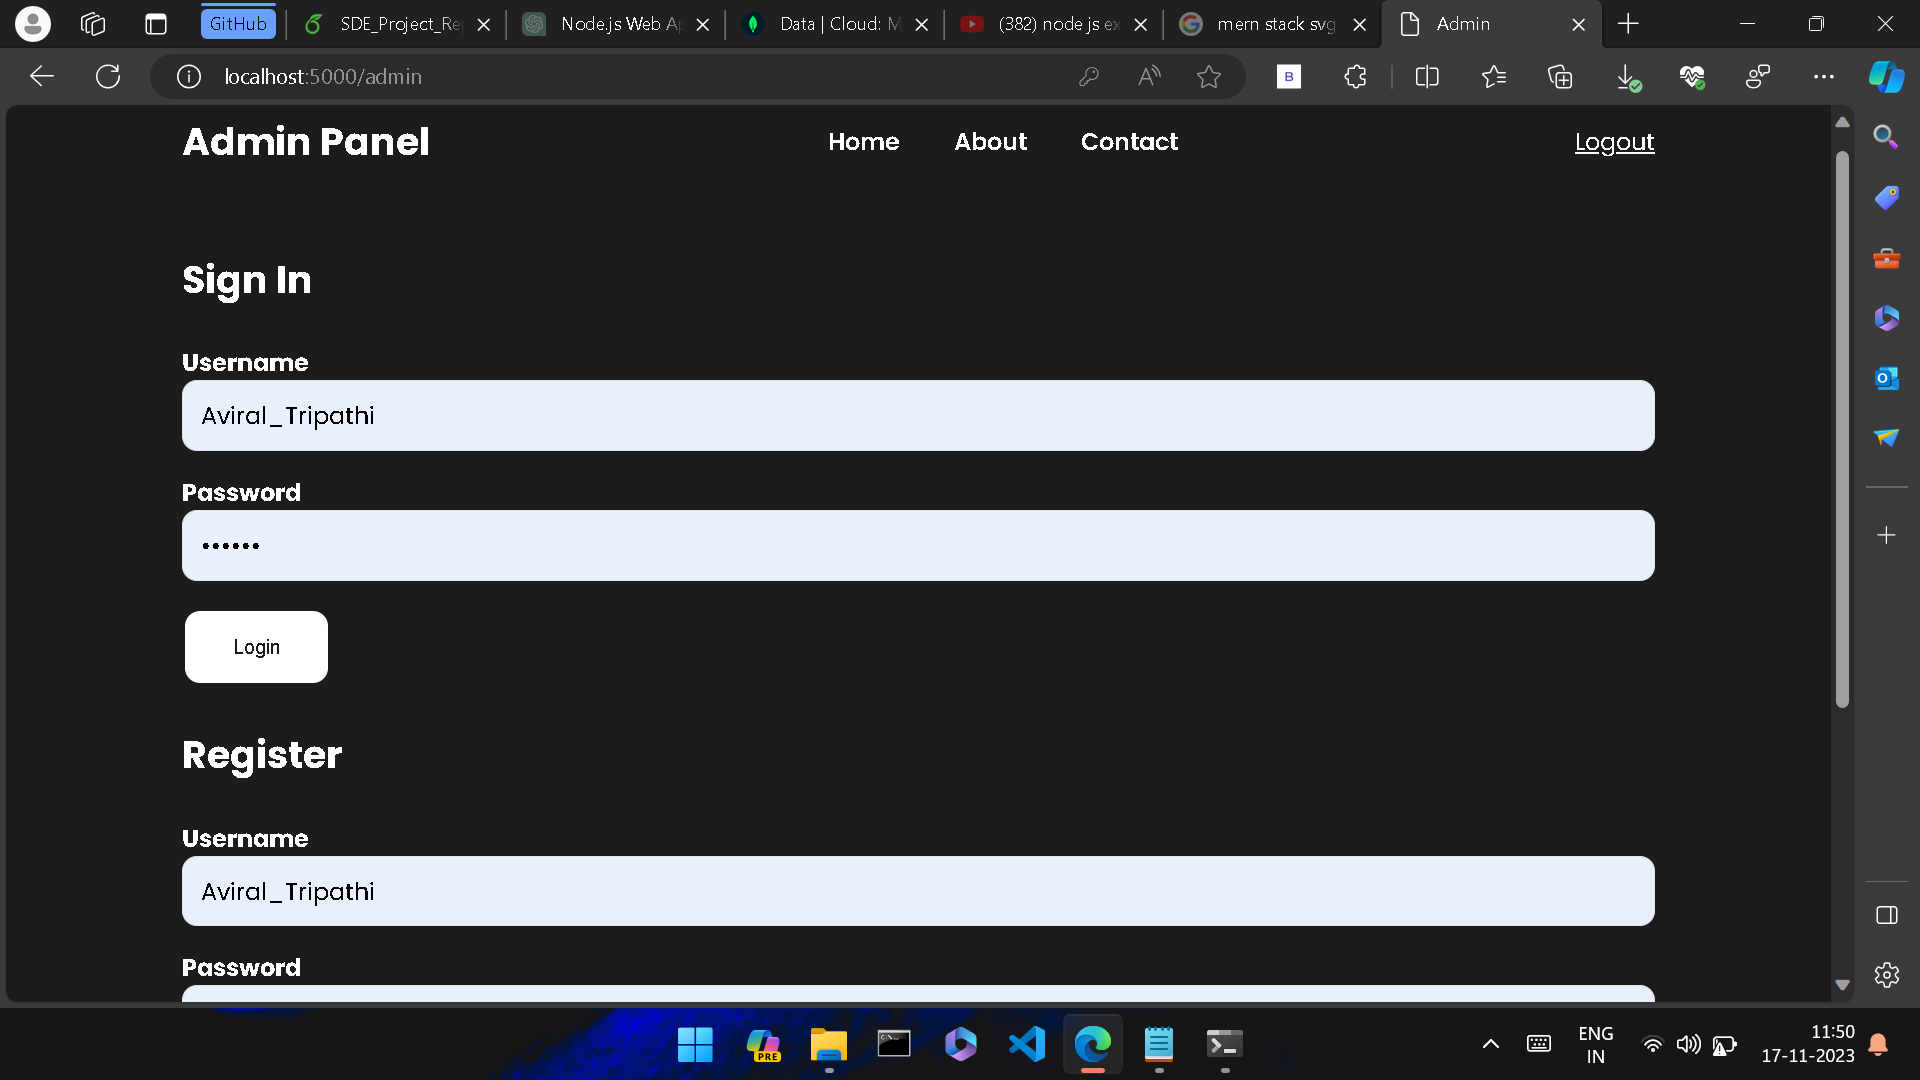
\includegraphics[width=1\textwidth]{assets/AdminPanel.png}
    \caption{Login and Registration forms}
    \label{fig:logo}
\end{figure}

\begin{figure}[H]
    \centering
    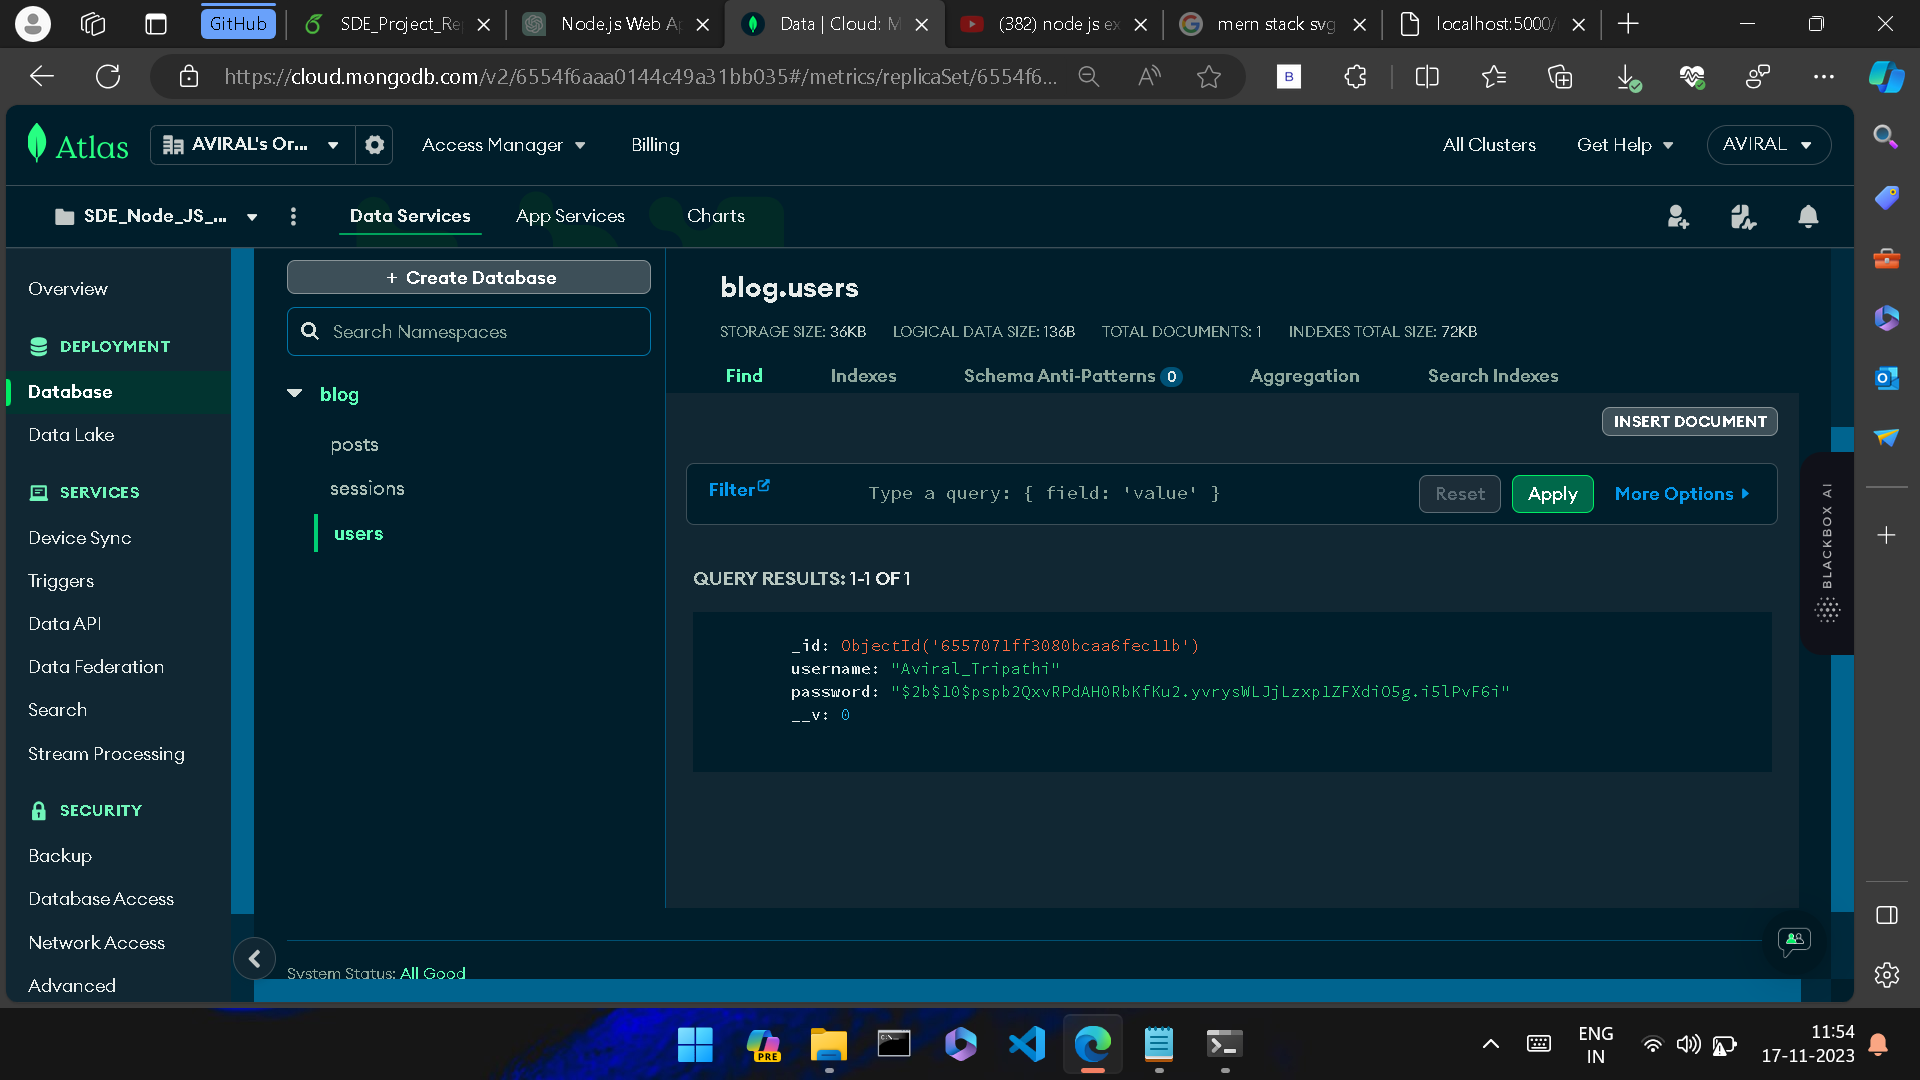
\includegraphics[width=1\textwidth]{assets/UsernameAndPasswordInMongoDB.png}
    \caption{Username and Password (Hashed) in Atlas}
    \label{fig:logo}
\end{figure}

Upon entering a registered username and password a user can login to 'create', 'edit', and 'delete' the existing posts in the blog.

\begin{figure}[H]
    \centering
    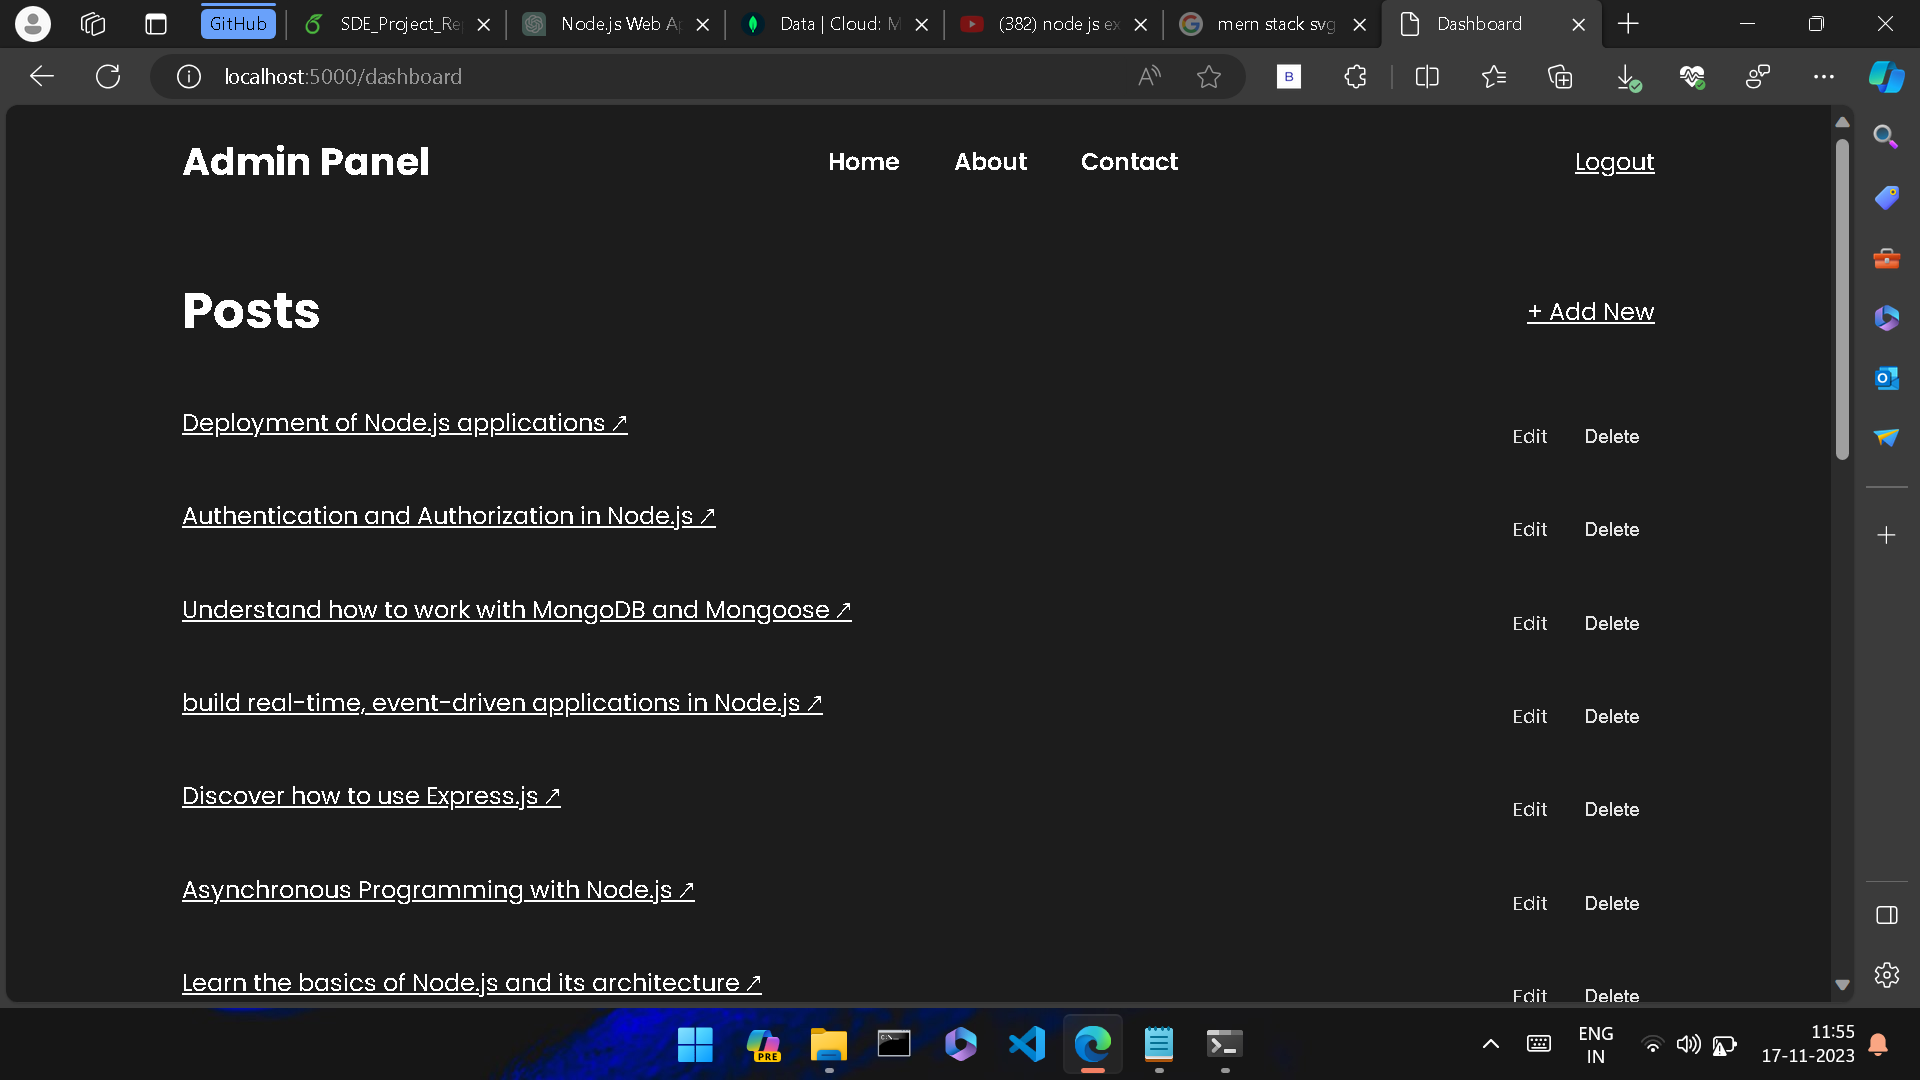
\includegraphics[width=1\textwidth]{assets/LoggedinUser.png}
    \caption{Loggedin User Dashboard}
    \label{fig:logo}
\end{figure}

\begin{figure}[H]
    \centering
    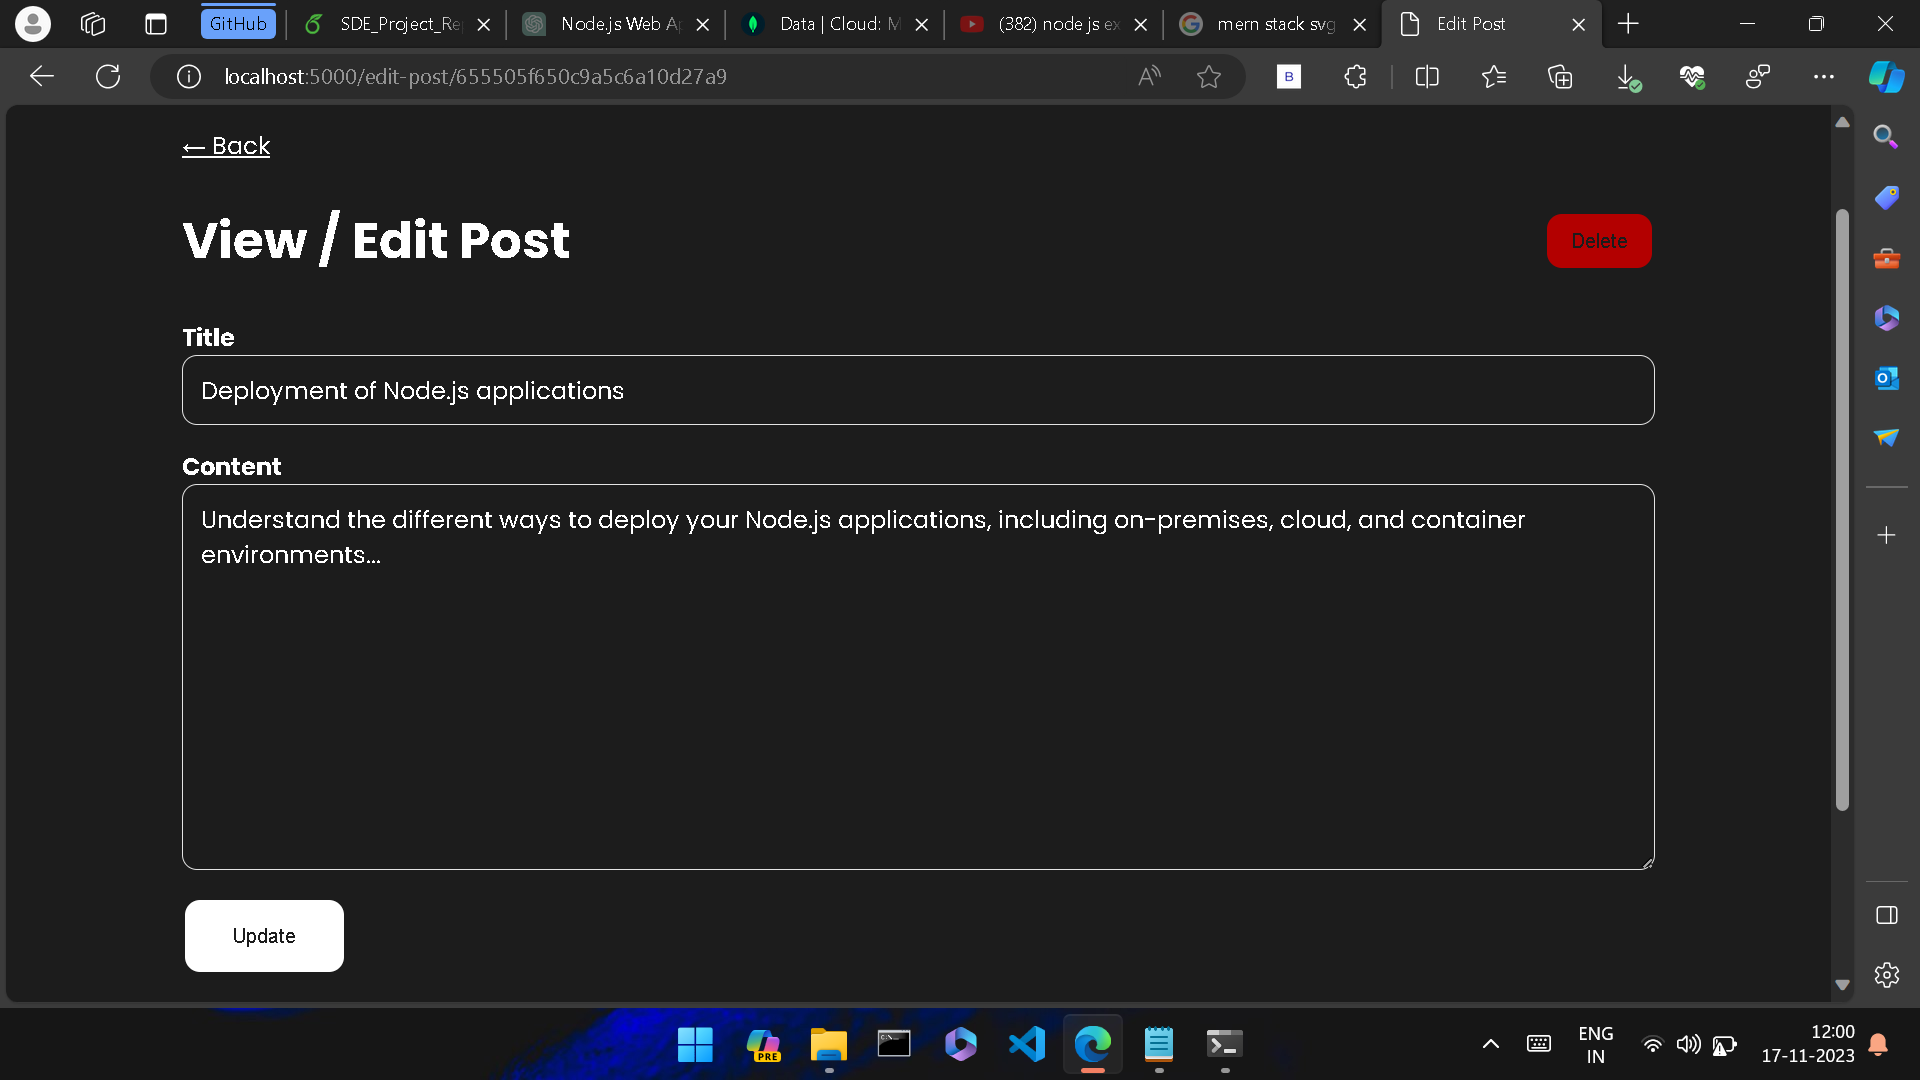
\includegraphics[width=1\textwidth]{assets/editOrDeletePost.png}
    \caption{Editing or deleting a post}
    \label{fig:logo}
\end{figure}

\begin{figure}[H]
    \centering
    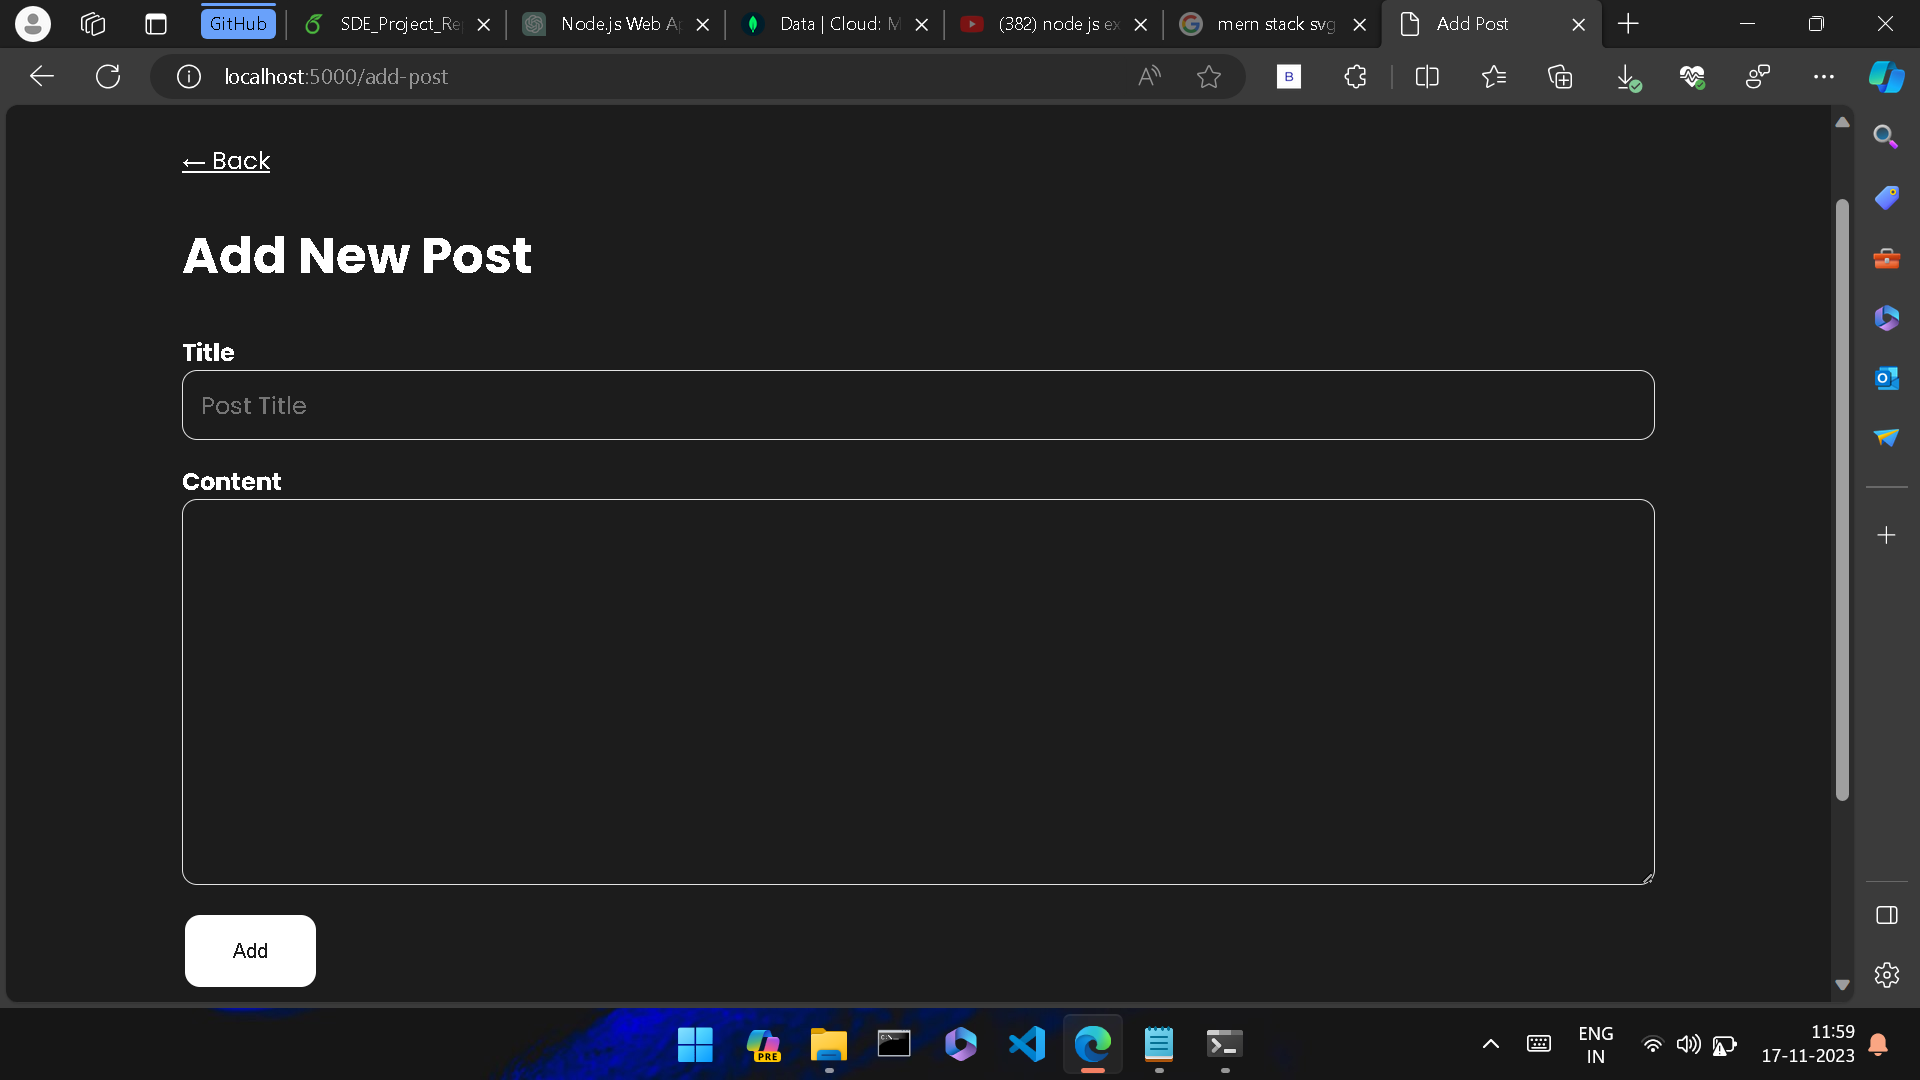
\includegraphics[width=1\textwidth]{assets/creatingAnewPost.png}
    \caption{Creating a post}
    \label{fig:logo}
\end{figure}


\clearpage

\section{GitHub Repository Link}

\begin{figure}[H]
    \centering
    \includegraphics[width=1\textwidth]{assets/GitHub-Mark-ea2971cee799.png}
    \caption{GitHub Link}
    \label{fig:logo}
\end{figure}

\textbf{\Large GitHub Repository Link}

\large
\url{https://github.com/AviralTripathim22ma012/NodeJS_MERN_Stack_Blog_SDE_Project/}

\clearpage

\section{References}



\begin{enumerate}[label=\arabic*.,itemsep=0pt,parsep=0pt]

      \item \url{https://youtu.be/-foo92lFIto?si=lXMIOPTFUxTwPkQ3}
      \item \url{https://youtu.be/gv3FFnOdCIo?si=BC4bG-fz92hbpfD1}
      \item \url{https://youtu.be/MruZEGPibC4?si=fxKXzWD3Dr-ge4Yj}
      \item \url{https://youtu.be/FjuctFNN0FA?si=PRQdkW1fHbEYRup5}
      \item \url{https://youtu.be/Cz-2QzkuCHo?si=m_25ddm7ogHtVHvy}
      \item \url{https://youtu.be/9Bnpl6bcev4?si=q5RistigoE2T_5Jo}
      \item \url{https://youtu.be/FmqBk2UTHzE?si=5tjSsXuZ762hO6ZV}
      \item \url{https://youtu.be/uCQirwe5UVg?si=sgsjaz5scrUxX3-b}
      \item \url{https://youtu.be/xQVM33SAjLM?si=pK3NygH6vzBZhLTp}
      \item \url{https://youtu.be/gR1Zlu4u58g?si=8LZwaFwg6PtB8Cjg}
      \item \url{https://youtu.be/eopdY_rD2FE?si=9vKcccGyZq1jX-lG}
      \item \url{https://youtu.be/bJSj1a84I20?si=Bo1HYyrHLdekqSC_}
      \item \url{https://youtu.be/1IX6qThkXJ4?si=XxS7sarJdUCh-g4Z}
      \item \url{https://youtu.be/zuye-dYSkS0?si=COq3QIzJiEtY3NFw}
      \item \url{https://youtu.be/TXJsBBK4Lhw?si=gnGgamkgmAJnw4dV}
      \item \url{https://youtu.be/R81g-2r6ynM?si=bgfT3gcz90hZAaXj}
      \item \url{https://youtu.be/JehgY5VOh5c?si=96CkhNHch0Pa1T-j}
      \item \url{https://www.youtube.com/watch?v=cQeCi2hT3is}
      \item \url{https://youtu.be/bJSj1a84I20?si=AsipUC19iwX9NR4r}
      \item \url{https://youtu.be/zQAdZYxbH14?si=VFRKGx3Exkt1d_k6}
      \item \url{https://youtu.be/xKs2IZZya7c?si=v-cgNS3OS3XS0Zql}
      \item \url{https://www.youtube.com/watch?v=FVnA1d_TGw0}
      \item \url{https://github.com/RaddyTheBrand/25.NodeJs-Express-EJS-MongoDB--Blog}
      \item \url{https://github.com/dejwid/mern-blog}
      \item \url{https://nodejs.org/en/download}
      \item \url{https://nodejs.org/en/learn/getting-started/how-to-install-nodejs}
      \item \url{https://react.dev/}
      \item \url{https://react.dev/learn}
      \item \url{https://chat.openai.com/}
      \item \url{https://www.mongodb.com/}
      \item \url{https://www.mongodb.com/products/tools/compass}
      \item \url{https://www.mongodb.com/try/download/compass}
      \item \url{https://www.mongodb.com/try/download/compass}
      \item \url{https://www.mongodb.com/try/download/atlascli}
      \item \url{https://www.mongodb.com/try/download/atlas-kubernetes-operator}
      \item \url{https://www.mongodb.com/try/download/mongosync}
    
    
\end{enumerate}


\clearpage

\listoffigures

\clearpage


\end{document}